\chapter[Fundamental Algorithms]{Fundamental\\ Algorithms}
\label{chap:fundamental_algorithms}

% Position the image to the right of the heading.
\vspace{-9\baselineskip} % move up
\hfill
 \begin{minipage}{0.5\textwidth}
 \centering
 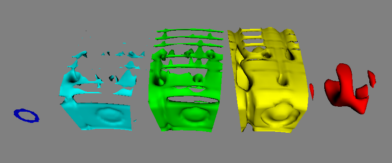
\includegraphics{VTKTextbook-54}
  \captionof*{figure}{\textit{Isosurfaces of a combustor dataset computed at multiple values.}}
 \end{minipage}
\vspace{2\baselineskip}

\firstletter{W}e have seen how to represent basic types of visualization data such as image data, structured grids, unstructured grids, and polygonal data.
This chapter explores methods to transform this data to and from these various representations, eventually generating graphics primitives that we can render.
These methods are called algorithms, and are of special interest to those working in the field of visualization.
Algorithms are the verbs that allow us to express our data in visual form.
By combining these verbs appropriately, we can reduce complex data into simple, readily comprehensible sentences that are the power of data visualization.

\section{Introduction}

The algorithms that transform data are the heart of data visualization.
To describe the various transformations available, we need to categorize algorithms according to the structure and type of transformation.
By structure we mean the effects that transformation has on the topology and geometry of the dataset.
By type we mean the type of dataset that the algorithm operates on.

Structural transformations can be classified in four ways, depending on how they affect the geometry, topology, and attributes of a dataset.

\begin{itemize}

\item \emph{Geometric transformations} alter input geometry but do not changed the topology of the dataset. For example, if we translate, rotate, and/or scale the points of a polygonal dataset, the topology does not change, but the point coordinates, and therefore the geometry, does.

\item \emph{Topological transformations} alter input topology but do not change geometry and attribute data. Converting a dataset type from polygonal data to unstructured grid data, or from image data to unstructured grid, changes the topology but not the geometry. More often, however, the geometry changes whenever the topology does, so topological transformation is uncommon.

\item \emph{Attribute transformations} convert data attributes from one form to another, or create new attributes from the input data. The structure of the dataset remains unaffected. Computing vector magnitude or creating scalars based on elevation are data attribute transformations.

\item \emph{Combined transformations} change both dataset structure and attribute data. For example, computing contour lines or surfaces is a combined transformation.

\end{itemize}

We also may classify algorithms according to the type of data they operate on, or the type of data they generate. By type, we most often mean the type of attribute data, such as scalars or vectors. Typical categories include:

\begin{itemize}

\item \emph{Scalar\index{algorithms!scalar} algorithms} operate on scalar data. For example, the generation of contour lines of temperature on a weather map.

\item \emph{Vector\index{algorithms!vector} algorithms} operate on vector data. Showing oriented arrows of airflow (direction and magnitude) is an example of vector visualization.

\item \emph{Tensor\index{algorithms!tensor} algorithms} operate on tensor matrices. An example of a tensor algorithm is to show the components of stress or strain in a material using oriented icons.

\item \emph{Modelling\index{algorithms!modelling} algorithms} generate dataset topology or geometry, or surface normals or texture data. Modelling algorithms tend to be the catch-all category for many algorithms, since some do not fit neatly into any single category mentioned above. For example, generating glyphs oriented according to the vector direction and then scaled according to the scalar value, is a combined scalar/vector algorithm. For convenience we classify such an algorithm as a modelling algorithm, because it does not fit squarely into any other category.

\end{itemize}

Algorithms also can be classified according to the type of data they process. This is the most common scheme found in the visualization literature. However, this scheme is not without its problems. Often the categories overlap, resulting in confusion. For example, a category (not mentioned above) is \emph{volume visualization}, which refers to the visualization of volume data (or in our terminology, image data). This category was initially created to describe the visualization of scalar data arranged on a volume, but more recently, vector (and even tensor) data has been visualized on a volume. Hence, we have to qualify our techniques to \emph{volume vector visualization}, or other potentially confusing combinations.

In the text that follows, we will use the attribute type classification scheme: scalar, vector, tensor, and modelling. In cases where the algorithms operate on a particular dataset type, we place them in the appropriate category according to our best judgment. Be forewarned, though, that alternative classification schemes do exist, and may be better suited to describing the true nature of the algorithm.

\begin{figure}[!htb]
	\centering
	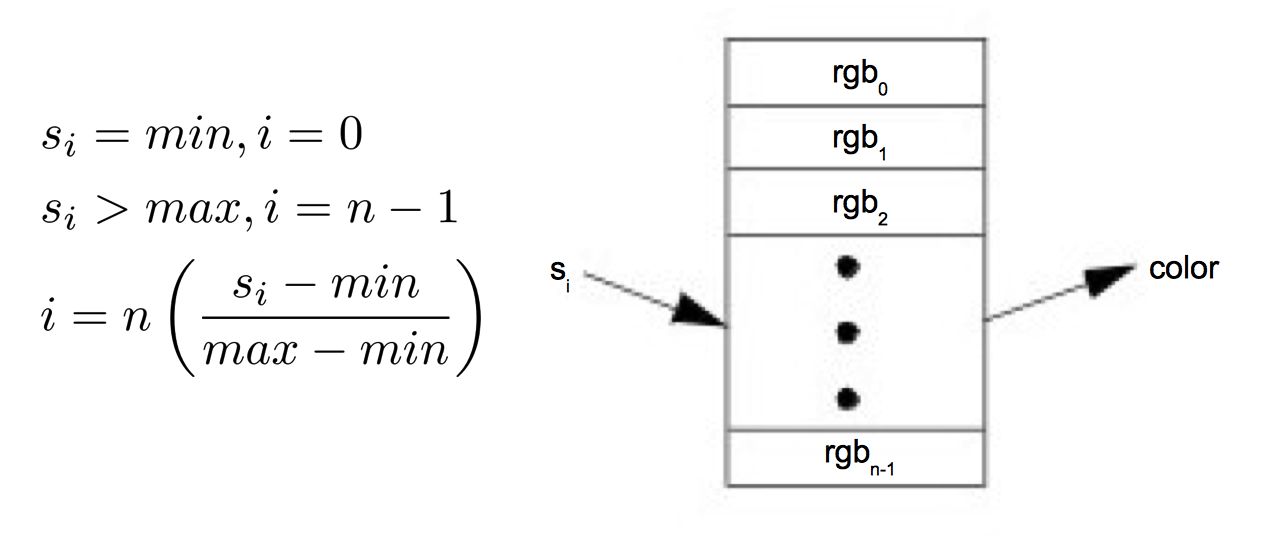
\includegraphics[width=0.8\textwidth]{Figure6-1}\\
	\caption{Mapping scalars to colors via a lookup table.}\label{fig:Figure6-1}
\end{figure}

\subsection{Generality Versus Efficiency}
\label{subsec:benerality_vs_efficiency}

Most algorithms can be written specifically for a particular dataset type, or more generally, treating any dataset type. The advantage of a specific algorithm is that it is usually faster than a comparable general algorithm. (See ``Other Data Abstractions'' on page \pageref{sec:other_data_abstractions} where we discussed the tradeoff between abstract and concrete forms.) An implementation of a specific algorithm also may be more memory efficient and its implementation may better reflect the relationship between the algorithm and the dataset type it operates on.

One example of this is contour surface creation. Algorithms for extracting contour surfaces were originally developed for volume data, mainly for medical applications. The regularity of volumes lends itself to efficient algorithms. However, the specialization of volume--based algorithms precludes their use for more general datasets such as structured or unstructured grids. Although the contour algorithms can be adapted to these other dataset types, they are less efficient than those for volume datasets.

Our presentation of algorithms favors the more general implementations. In some special cases we will describe performance improving techniques for particular dataset types. Refer to the bibliography at the end of each chapter for detailed descriptions of specialized algorithms.

\section{Scalar Algorithms}
\index{algorithms!scalar|(}

Scalars are single data values associated with each point and/or cell of a dataset. (Recall that in the \emph{Visualization Toolkit} we associate data with points.) Because scalar data is commonly found in real--world applications, and because scalar data is so easy to work with, there are many different algorithms to visualize it.

\subsection{Color Mapping}
\label{subsec:color_mapping}
\index{color mapping|(}

\emph{Color mapping} is a common scalar visualization technique that maps scalar data to colors, and displays the colors on the computer system. The scalar mapping is implemented by indexing into a \emph{color lookup table}\index{lookup table}. Scalar values serve as indices into the lookup table.

The mapping proceeds as follows. The lookup table holds an array of colors (e.g., red, green, blue components or other comparable representations). Associated with the table is a minimum and maximum \emph{scalar range (min, max)} into which the scalar values are mapped. Scalar values greater than the maximum range are clamped to the maximum color, scalar values less than the minimum range are clamped to the minimum color value. Then, for each scalar value $x_i$, the index $i$ into the color table with n entries (and 0--offset) is given by Figure \ref{fig:Figure6-1}.

A more general form of the lookup table is called a transfer function. A transfer function is any expression that maps scalar values into a color specification. For example, Figure \ref{fig:Figure6-2} maps scalar values into separate intensity values for the red, green, and blue color components. We can also use transfer functions to map scalar data into other information such as local transparency. (Transfer functions are discussed in more detail in ``Transparency and Alpha Values'' on page \pageref{sec:transparency_alpha} and ``Volume Rendering'' on page \pageref{sec:volume_rendering}).
A lookup table is a discrete sampling of a transfer function.
We can create a lookup table from any transfer function by sampling the transfer function at a set of discrete points.

Color mapping is a one--dimensional visualization technique. It maps one piece of information (i.e., a scalar value) into a color specification. However, the display of color information is not limited to one-dimensional displays. Often we use color information mapped onto 1D, 2D, or 3D objects. This is a simple way to increase the information content of our visualizations.

The key to color mapping for scalar visualization is to choose the lookup table entries carefully. Figure \ref{fig:Figure6-3} shows four different lookup tables used to visualize gas density as fluid flows through a combustion chamber. The first lookup table is gray-scale. Grayscale tables often provide better structural detail to the eye. The other three images in Figure \ref{fig:Figure6-3} uses different colored lookup tables. The second uses rainbow hues from blue to red. The third uses rainbow hues arranged from red to blue. The last table uses a table designed to enhance contrast. Careful use of colors can often enhance important features of a dataset. However, any type of lookup table can exaggerate unimportant details or create visual artifacts because of unforeseen interactions between data, color choice, and human physiology.

Designing lookup tables is as much art as it is science. From a practical point of view, tables should accentuate important features, while minimizing less important or extraneous details. It is also desirable to use palettes that inherently contain scaling information. For example, a color rainbow scale from blue to red is often used to represent temperature scale, since many people associate ``blue'' with cold temperatures, and ``red'' with hot temperatures. However, even this scale is problematic: a physicist would say that blue is hotter than red, since hotter objects emit more blue light (i.e., shorter wavelength) than red. Also, there is no need to limit ourselves to ``linear'' lookup tables. Even though the mapping of scalars into colors has been presented as a linear operation (Figure \ref{fig:Figure6-1}, the table itself need not be linear. That is, tables can be designed to enhance small variations in scalar value using logarithmic or other schemes, improving the comfort level and engaging the human observer more deeply in the presentation of data improves the effectiveness of communication.

\begin{figure}[!htb]
	\centering
	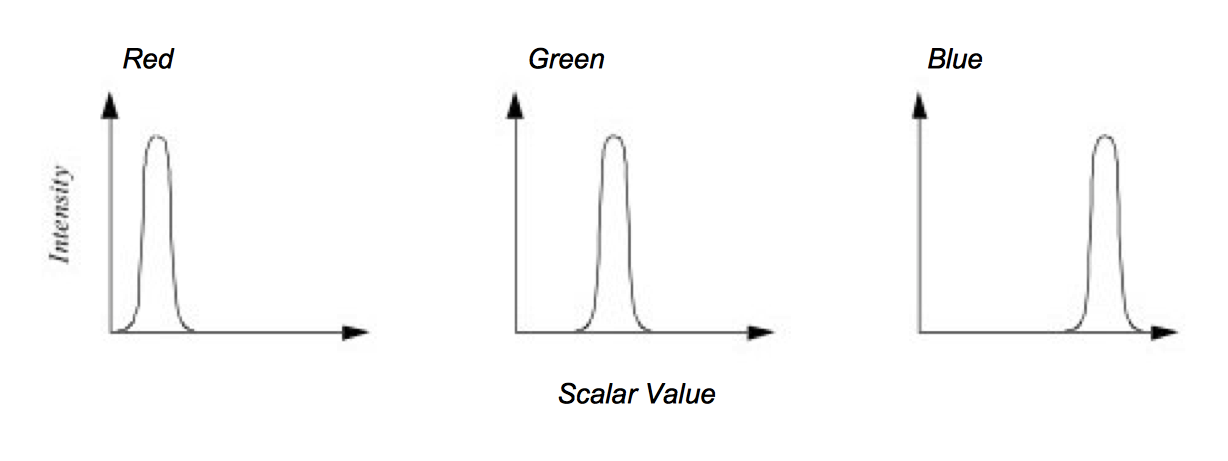
\includegraphics[width=0.8\textwidth]{Figure6-2}
	\caption{Transfer function for color components red, green and blue as a function of scalar value.}
	\label{fig:Figure6-2}
\end{figure}

\begin{figure}[!htb]
	\centering
	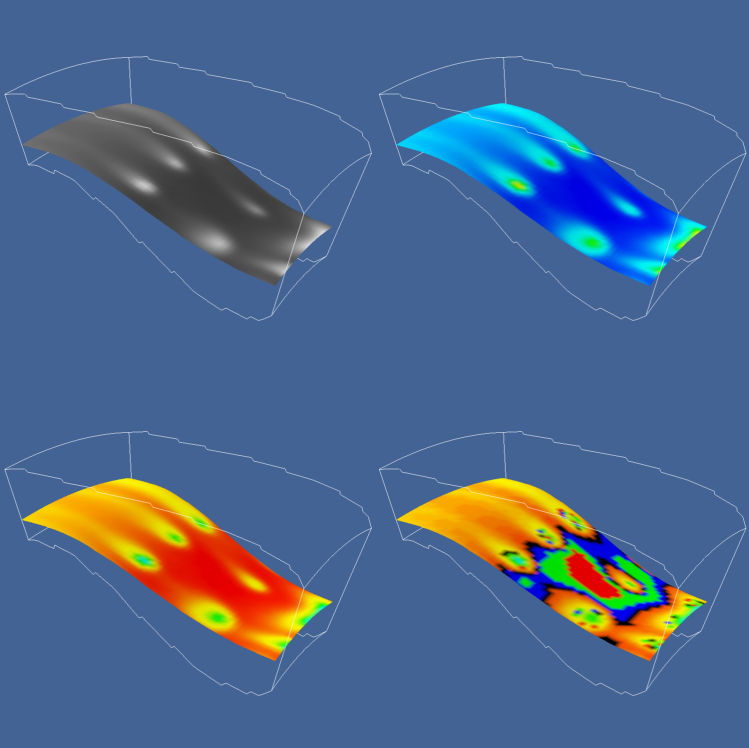
\includegraphics[width=0.8\textwidth]{Figure6-3}
	\caption{Flow density colored with different lookup tables. Top-left: grayscale; Top-right rainbow (blue to red); lower-left rainbow (red to blue); lower-right large contrast. (\href{https://lorensen.github.io/VTKExamples/site/Cxx/Rendering/Rainbow/}{Rainbow.cxx}) and (\href{https://lorensen.github.io/VTKExamples/site/Python/Rendering/Rainbow/}{Rainbow.py})}
	\label{fig:Figure6-3}
\end{figure}
\index{color mapping|)}

\subsection{Contouring}
\label{subsec:contouring}
\index{contouring|(}

A natural extension to color mapping is \emph{contouring}. When we see a surface colored with data values, the eye often separates similarly colored areas into distinct regions. When we contour data, we are effectively constructing the boundary between these regions. These boundaries correspond to contour lines (2D) or surfaces (3D) of constant scalar value.

Examples of 2D contour displays include weather maps annotated with lines of constant temperature (isotherms), or topological maps drawn with lines of constant elevation. Three-dimensional contours are called \emph{isosurfaces}\index{isosurface}, and can be approximated by many polygonal primitives. Examples of isosurfaces include constant medical image intensity corresponding to body tissues such as skin, bone, or other organs. Other abstract isosurfaces such as surfaces of constant pressure or temperature in fluid flow also may be created.


\begin{figure}[!htb]
	\centering
	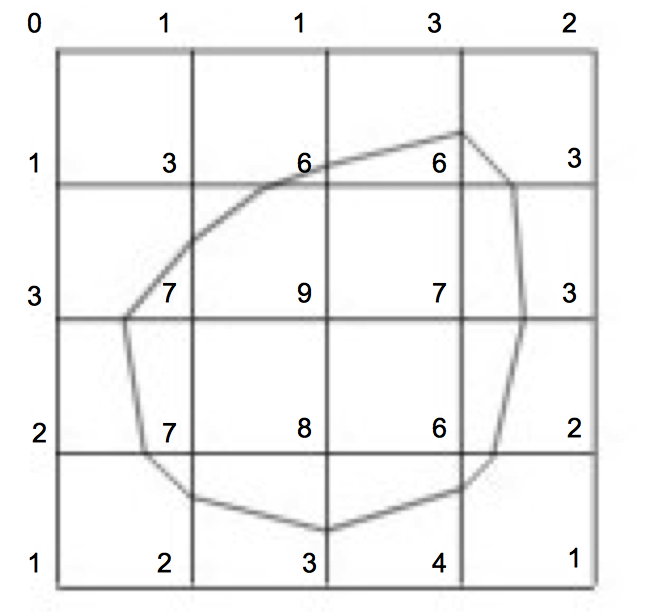
\includegraphics[width=0.8\textwidth]{Figure6-4}
	\caption{ Contouring a 2D stuctured grid with contour line value = 5.}
	\label{fig:Figure6-4}
\end{figure}

Consider the 2D structured grid shown in Figure \ref{fig:Figure6-4}. Scalar values are shown next to the points that define the grid. Contouring always begins by selecting a scalar value, or contour value, that corresponds to the contour lines or surfaces generated. To generate the contours, some form of interpolation must be used. This is because we have scalar values at a finite set of points in the dataset, and our contour value may lie between the point values. Since the most common interpolation technique is linear, we generate points on the contour surface by linear interpolation along the edges. If an edge has scalar values 10 and 0 at its two endpoints, and if we are trying to generate a contour line of value 5, then edge interpolation computes that the contour passes through the midpoint of the edge.

Once the points on cell edges are generated, we can connect these points into contours using a few different approaches. One approach detects an edge intersection (i.e., the contour passes through an edge) and then ``tracks'' this contour as it moves across cell boundaries. We know that if a contour edge enters a cell, it must exit a cell as well. The contour is tracked until it closes back on itself, or exits a dataset boundary. If it is known that only a single contour exists, then the process stops. Otherwise, every edge in the dataset must be checked to see whether other contour lines exist.

Another approach uses a divide and conquer technique, treating cells independently. This is the \emph{marching squares} algorithm in 2D, and \emph{marching cubes}\index{marching cubes|(} \cite{Lorensen87} in 3D. The basic assumption of these techniques is that a contour can only pass through a cell in a finite number of ways. A case table is constructed that enumerates all possible topological \emph{states} of a cell, given combinations of scalar values at the cell points. The number of topological states depends on the number of cell vertices, and the number of inside / outside relationships a vertex can have with respect to the contour value. A vertex is considered inside a contour if its scalar value is larger than the scalar value of the contour line. Vertices with scalar values less than the contour value are said to be outside the contour. For example, if a cell has four vertices and each vertex can be either inside or outside the contour, there are $2^4 = 16$ possible ways that the contour passes through the cell. In the case table we are not interested in where the contour passes through the cell (e.g., geometric intersection), just how it passes through the cell (i.e., topology of the contour in the cell).

Figure \ref{fig:Figure6-5} shows the sixteen combinations for a square cell. An index into the case table can be computed by encoding the state of each vertex as a binary digit. For 2D data represented on a rectangular grid, we can represent the 16 cases with 4 bit index. Once the proper case is selected, the location of the contour line / cell edge intersection can be calculated using interpolation. The algorithm processes a cell and then moves, or \emph{marches t} o the next cell. After all cells are visited, the contour will be completed. In summary, the marching algorithms proceed as follows:

\begin {enumerate}

\item Select a cell.

\item Calculate the inside / outside state of each vertex of the cell.

\item Create an index by storing the binary state of each vertex in a separate bit.

\item Use the index to look up the topological state of the cell in a case
table.

\item Calculate the contour location (via interpolation) for each edge in  the case table.

\end{enumerate}

This procedure will construct independent geometric primitives in each cell. At the cell boundaries duplicate vertices and edges may be created. These duplicates can be eliminated by using a special coincident point merging operation. Note that interpolation along each edge should be done in the same direction. If not, numerical roundoff will likely cause points to be generated that are not precisely coincident, and will not merge properly.

There are advantages and disadvantages to both the edge--tracking and marching cubes approaches. The marching squares algorithm is easy to implement. This is particularly important when we extend the technique into three dimensions, where isosurface tracking becomes much more difficult. On the other hand, the algorithm creates disconnected line segments and points, and the required merging operation requires extra computation resources. The tracking algorithm can be implemented to generate a single polyline per contour line, avoiding the need to merge coincident points.

\begin{figure}[!htb]
\centering
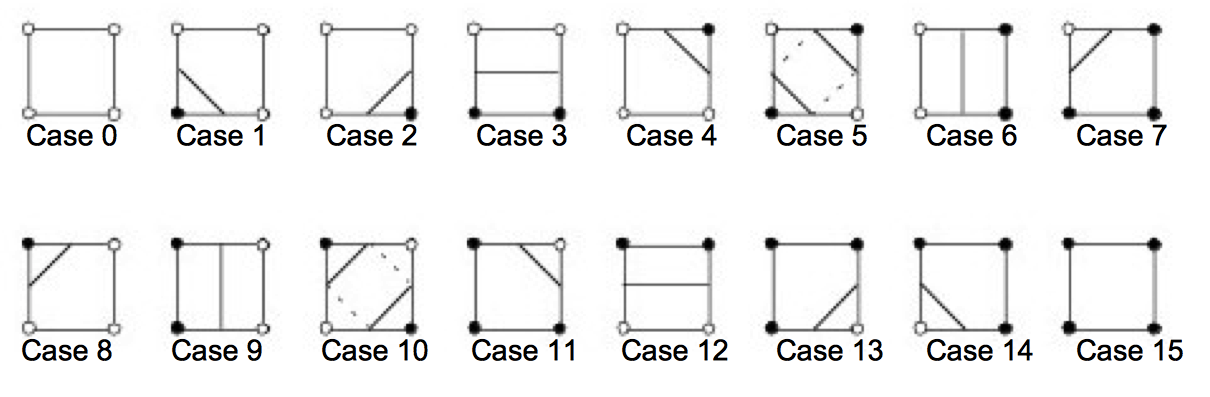
\includegraphics[width=0.8\textwidth]{Figure6-5}\\
\caption{ Sixteen different marching squares cases. Dark vertices indicate scalar value is above contour value. Cases 5 and 10 are ambiguous.}
\label{fig:Figure6-5}
\end{figure}


\begin{figure}[!htb]
	\centering
	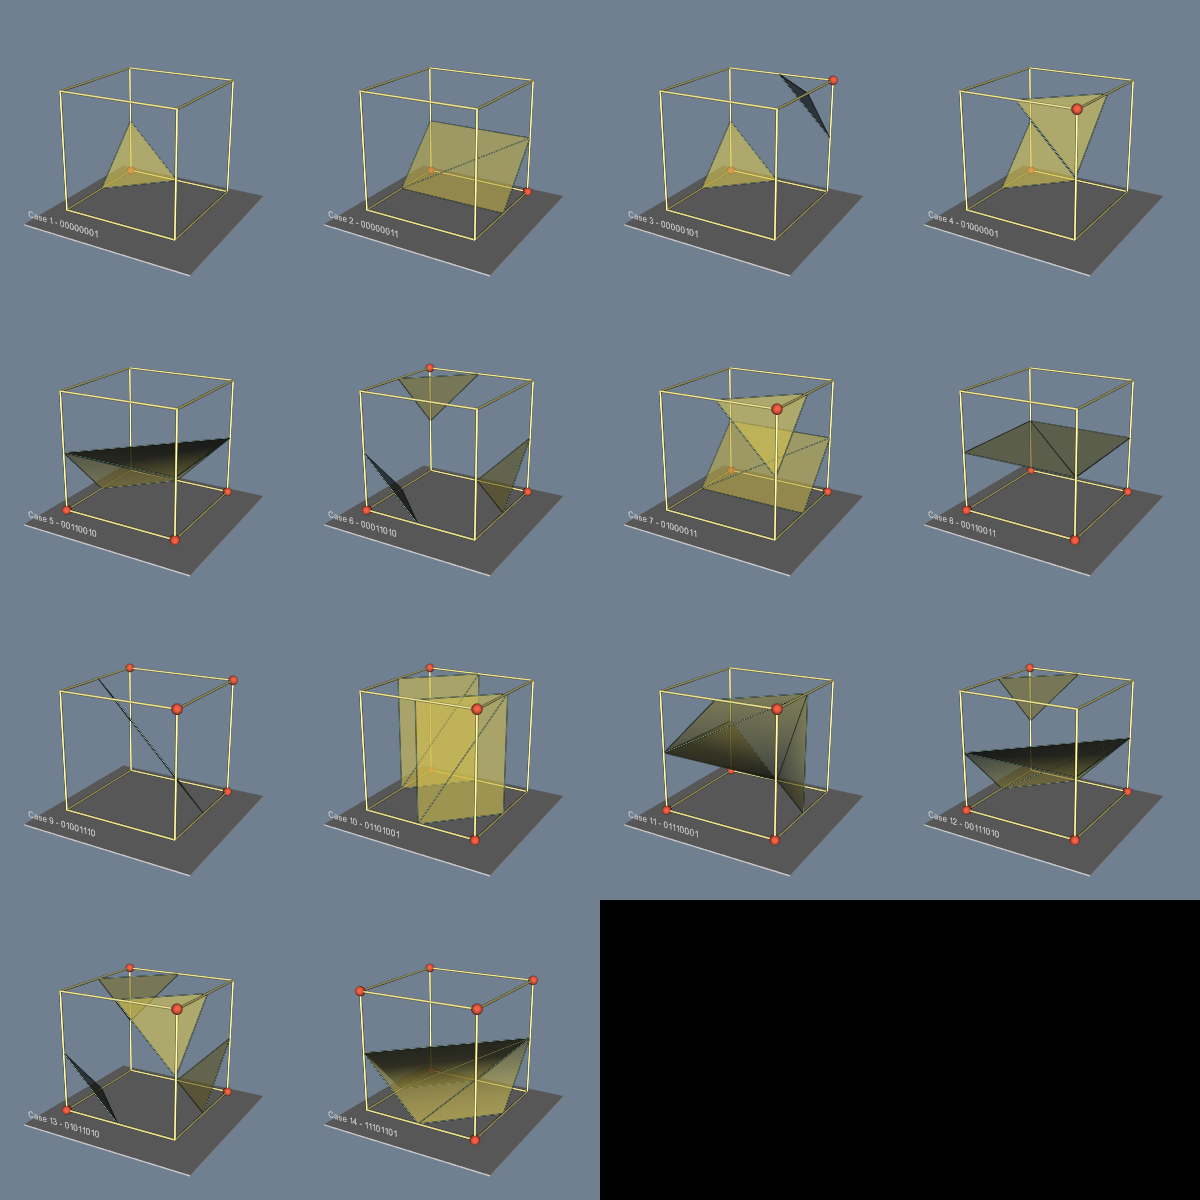
\includegraphics[width=0.8\textwidth]{Figure6-6}\\
	\caption{Marching Cubes cases\index{marching cubes!cases} for 3D isosurface generation. The 256 possible cases have been reduced to 15 cases using symmetry. Red vertices are greater than the selected isosurface value. (\href{https://lorensen.github.io/VTKExamples/site/Cxx/VisualizationAlgorithms/MarchingCasesA/}{MarchingCasesA.cxx}) and (\href{https://lorensen.github.io/VTKExamples/site/Python/VisualizationAlgorithms/MarchingCasesA/}{MarchingCasesA.py})}
	\label{fig:Figure6-6}
\end{figure}


\begin{figure}[!htb]
	\centering
	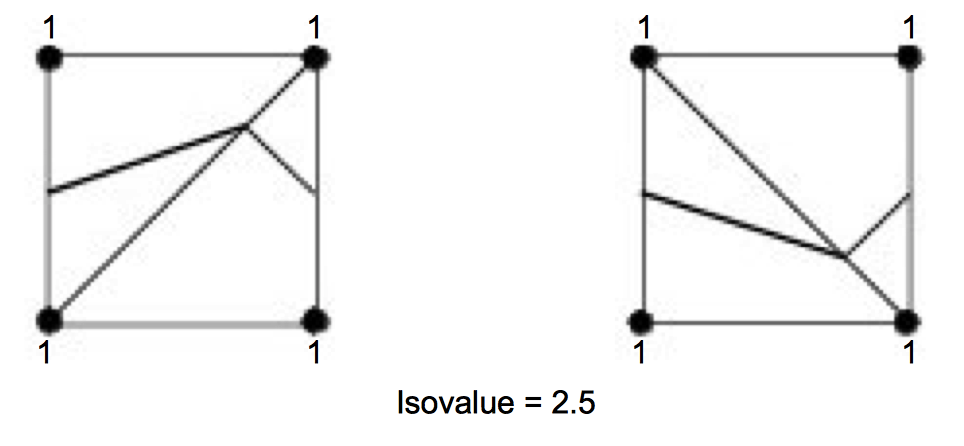
\includegraphics[width=0.8\textwidth]{Figure6-7}\\
	\caption{Using marching triangles or marching tetrahedra to resolve ambiguous cases on rectangular lattice (only face of cube is shown). Choice of diagonal orientation may result in ``bumps'' in contour surface. In 2D, diagonal orientation can be chosen arbitrarily, but in 3D diagonal is constrained by neighbor.}
	\label{fig:Figure6-7}
\end{figure}

As mentioned previously, the 3D analogy of marching squares is marching cubes. Here, there are 256 different combinations of scalar value, given that there are eight points in a cubical cell (i.e., $2^8$ combinations). Figure \ref{fig:Figure6-6} shows these combinations reduced to 15 cases\index{marching cubes!cases} by using arguments of symmetry. We use combinations of rotation and mirroring to produce topologically equivalent cases.

In two dimensions, contour ambiguity is simple to treat: for each ambiguous case we implement one of the two possible cases. The choice for a particular case is independent of all other choices. Depending on the choice, the contour may either extend or break the current contour as illustrated in Figure \ref{fig:Figure6-9}. Either choice is acceptable since the resulting contour lines will be continuous and closed (or will end at the dataset boundary).

In three dimensions the problem is more complex. We cannot simply choose an ambiguous case independent of all other ambiguous cases. For example Figure \ref{fig:Figure6-9} shows what happens if we carelessly implement two cases independent of one another. In this figure we have used the usual case 3 but replaced case 6 with its \emph{complementary} case. Complementary cases\index{marching cubes!complementary cases} are formed by exchanging the ``dark'' vertices with ``light'' vertices. (This is equivalent to swapping vertex scalar value from above the isosurface value to below the isosurface value, and vice versa.) The result of pairing these two cases is that a hole is left in the isosurface.

Several different approaches have been taken to remedy this problem. One approach tessellates the cubes with tetrahedron, and uses a \emph{marching tetrahedra} technique. This works because the marching tetrahedra exhibit no ambiguous cases. Unfortunately, the marching tetrahedra algorithm generates isosurfaces consisting of more triangles, and the tessellation of a cube with tetrahedra requires making a choice regarding the orientation of the tetrahedra. This choice may result in artificial ``bumps'' in the isosurface because of interpolation along the face diagonals as shown in Figure \ref{fig:Figure6-7}. Another approach evaluates the asymptotic behavior of the surface, and then chooses the cases to either join or break the contour. Nielson and Hamann \cite{Nielson91} have developed a technique based on this approach they call the \emph{asymptotic decider}. It is based on an analysis of the variation of the scalar variable across an ambiguous face. The analysis determines how the edges of isosurface polygons should be connected.

\begin{figure}[!htb]
	\centering
	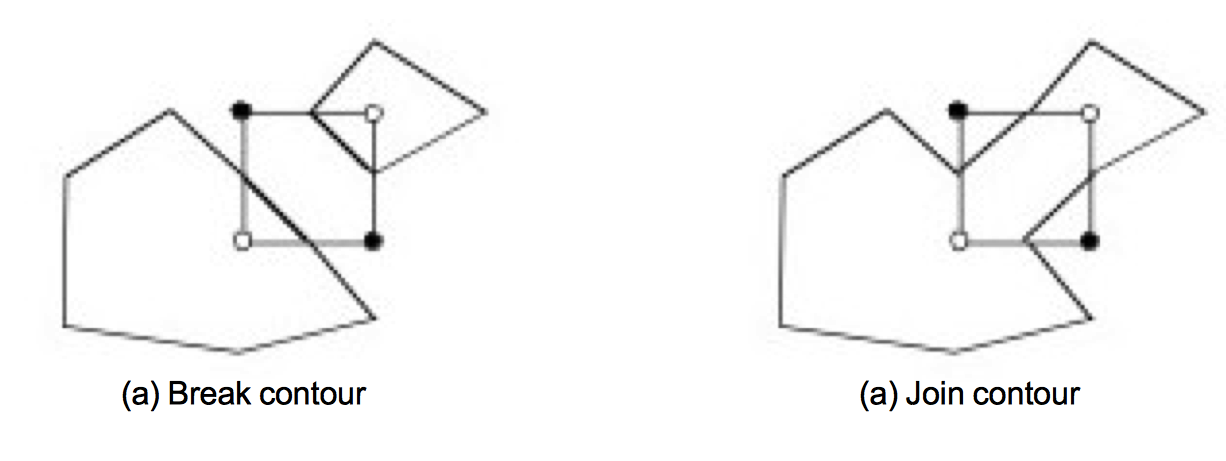
\includegraphics[width=0.8\textwidth]{Figure6-8}\\
	\caption{Choosing a particular contour case will break (a) or join (b) the current contour. Case shown is marching squares case 10.}
	\label{fig:Figure6-8}
\end{figure}

\begin{figure}[!htb]
	\centering
	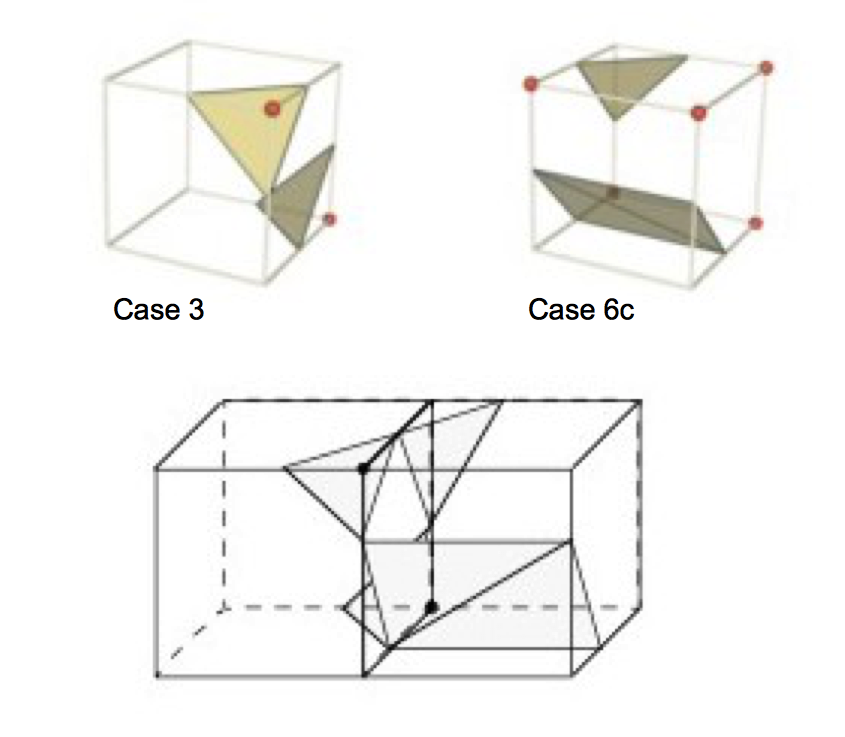
\includegraphics[width=0.8\textwidth]{Figure6-9}\\
	\caption{Arbitrarily choosing marching cubes cases leads to holes in the isosurface.}
	\label{fig:Figure6-9}
\end{figure}

A simple and effective solution extends the original 15 marching cubes cases by adding additional complementary cases. These cases are designed to be compatible with neighboring cases and prevent the creation of holes in the isosurface. There are six complementary cases required, corresponding to the marching cubes cases 3, 6, 7, 10, 12, and 13. The complementary marching cubes cases are shown in Figure \ref{fig:Figure6-10}.

\begin{figure}[!htb]
	\centering
	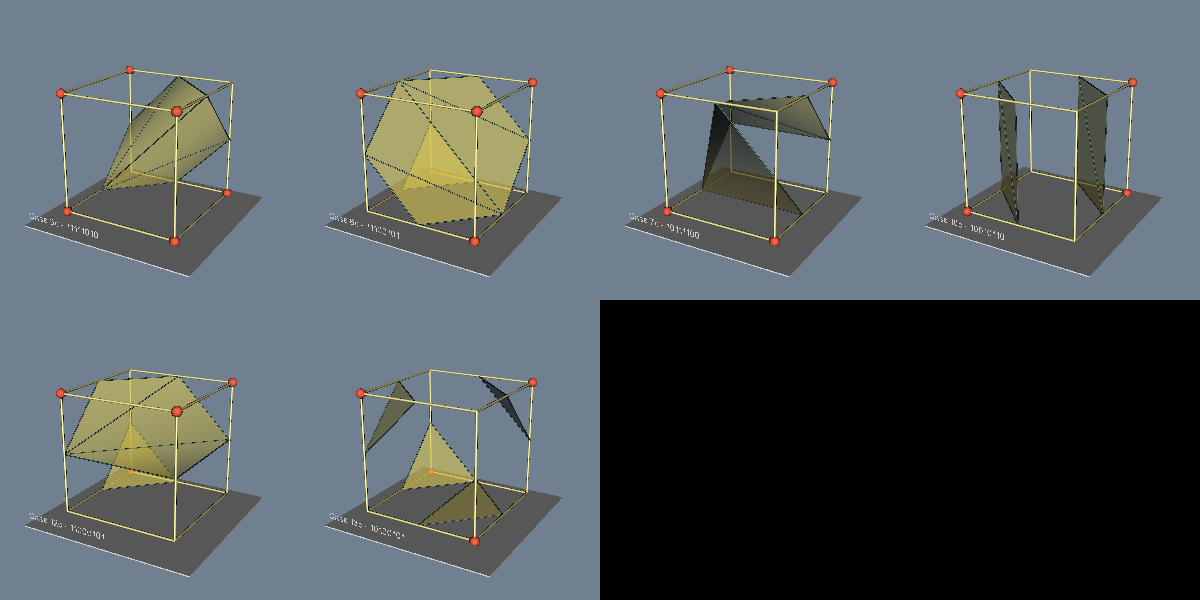
\includegraphics[width=0.8\textwidth]{Figure6-10}\\
	\caption{Marching cubes complementary cases\index{marching cubes!complementary cases}.(\href{https://lorensen.github.io/VTKExamples/site/Cxx/VisualizationAlgorithms/MarchingCasesB/}{MarchingCasesB.cxx}) and (\href{https://lorensen.github.io/VTKExamples/site/Python/VisualizationAlgorithms/MarchingCasesB/}{MarchingCasesB.py})}
	\label{fig:Figure6-10}
\end{figure}

We can extend the general approach of marching squares and marching cubes to other topological types. In VTK we use marching lines, triangles, and tetrahedra to contour cells of these types (or composite cells that are composed of these types). In addition, although we speak of regular types such as squares and cubes, marching cubes can be applied to any cell type topologically equivalent to a cube (e.g., hexahedron or non--cubical voxel).

Figure \ref{fig:Figure6-11} shows four applications of contouring. In Figure \ref{fig:Figure6-11a} we see 2D contour lines of CT density value corresponding to different tissue types. These lines were generated using marching squares. Figure \ref{fig:Figure6-11b} through Figure \ref{fig:Figure6-11d} are isosurfaces created by marching cubes. Figure \ref{fig:Figure6-11b} is a surface of constant image intensity from a computed tomography (CT) Xray imaging system. ( Figure \ref{fig:Figure6-11a} is a 2D subset of this data.) The intensity level corresponds to human bone. Figure \ref{fig:Figure6-11c} is an isosurface of constant flow density. Figure \ref{fig:Figure6-11d} is an isosurface of electron potential of an iron protein molecule. The image shown in Figure \ref{fig:Figure6-11b} is immediately recognizable because of our familiarity with human anatomy. However, for those practitioners in the fields of computational fluid dynamics and molecular biology, Figure \ref{fig:Figure6-11c} and Figure \ref{fig:Figure6-11d} are equally familiar. As these examples show, methods for contouring are powerful yet general techniques for visualizing data from a variety of fields.

\begin{figure}[htb]
	\begin{subfigure}[h]{0.48\linewidth}
		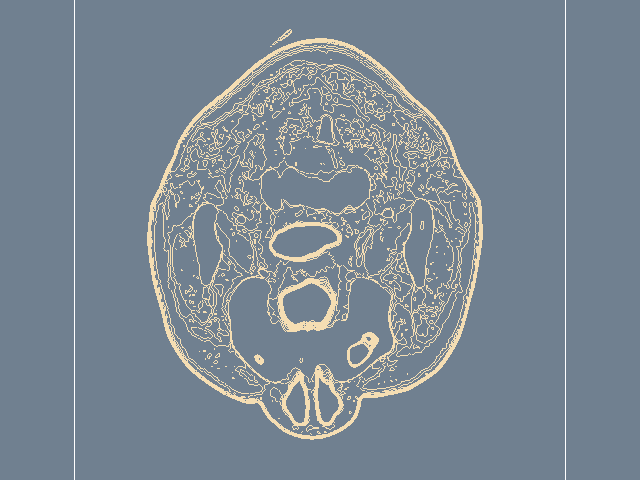
\includegraphics[width=\linewidth]{Figure6-11a}
		\caption{Marching squares used to generate contour lines.(\href{https://lorensen.github.io/VTKExamples/site/Cxx/VisualizationAlgorithms/HeadSlice}{HeadSlice.cxx} or \href{https://lorensen.github.io/VTKExamples/site/Python/VisualizationAlgorithms/HeadSlice/}{HeadSlice.py})}\label{fig:Figure6-11a}
	\end{subfigure}
	\hfill
	\begin{subfigure}[h]{0.48\linewidth}
		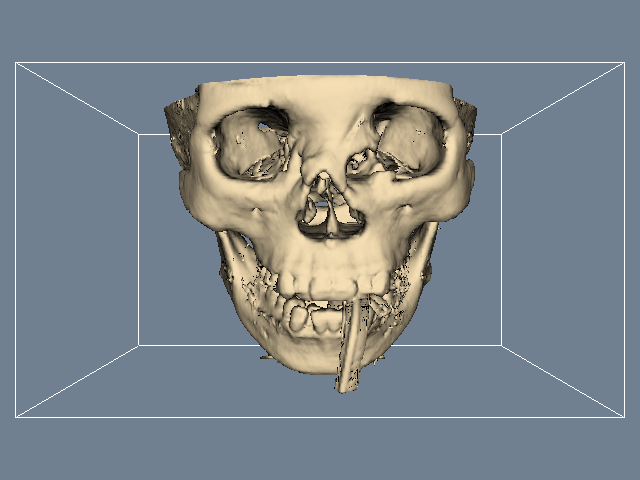
\includegraphics[width=\linewidth]{Figure6-11b}
		\caption{Marching Cubes surface of human bone\index{marching cubes!example}.(\href{https://lorensen.github.io/VTKExamples/site/Cxx/VisualizationAlgorithms/HeadBone}{HeadBone.cxx} or \href{https://lorensen.github.io/VTKExamples/site/Python/VisualizationAlgorithms/HeadBone/}{HeadBone.py})}\label{fig:Figure6-11b}
	\end{subfigure}%
	\hfill
	\begin{subfigure}[h]{0.48\linewidth}
		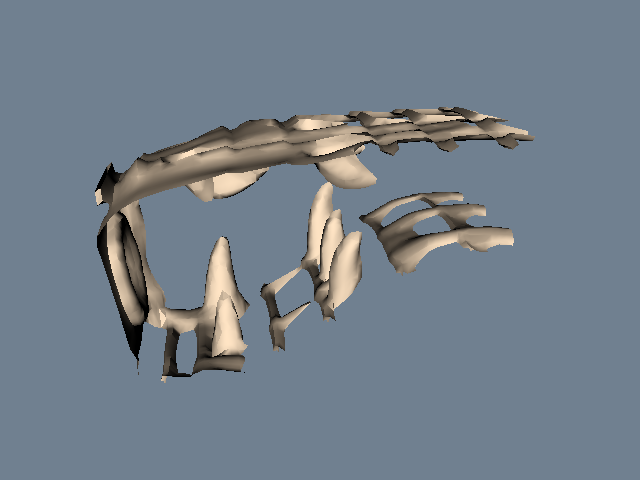
\includegraphics[width=\linewidth]{Figure6-11c}
		\caption{Marching squares used to generate contour lines.(\href{https://lorensen.github.io/VTKExamples/site/Cxx/VisualizationAlgorithms/CombustorIsosurface}{CombustorIsosurface.cxx} or \href{https://lorensen.github.io/VTKExamples/site/Python/VisualizationAlgorithms/CombustorIsosurface/}{CombustorIsosurface.py})}\label{fig:Figure6-11c}
	\end{subfigure}
	\hfill
	\begin{subfigure}[h]{0.48\linewidth}
		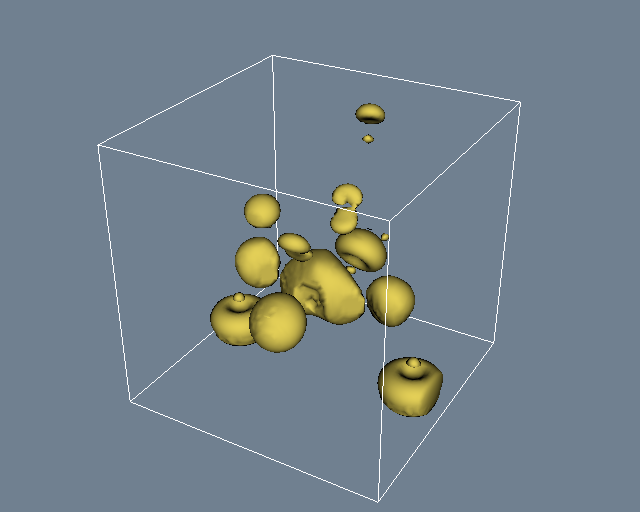
\includegraphics[width=\linewidth]{Figure6-11d}
		\caption{Marching Cubes surface of iron protein.(\href{https://lorensen.github.io/VTKExamples/site/Cxx/VisualizationAlgorithms/IronIsoSurface}{IronIsoSurface.cxx} or \href{https://lorensen.github.io/VTKExamples/site/Python/VisualizationAlgorithms/IronIsoSurface/}{IronIsoSurface.py})}\label{fig:Figure6-11d}
	\end{subfigure}%
	\caption{Contouring examples.}\label{fig:Figure6-11}
\end{figure}
\index{contouring|)}\index{marching cubes|)}

\subsection{Scalar Generation}
\label{subsec:scalar_generation}

The two visualization techniques presented thus far, color mapping and contouring, are simple, effective methods to display scalar information. It is natural to turn to these techniques first when visualizing data. However, often our data is not in a form convenient to these techniques. The data may not be single--valued (i.e., a scalar), or it may be a mathematical or other complex relationship. That is part of the fun and creative challenge of visualization: We must tap our creative resources to convert data into a form we can visualize.

For example, consider terrain data. We assume that the data is \emph{xyz} coordinates, where \emph{x} and \emph{y} represent the coordinates in the plane, and \emph{z} represents the elevation above sea level. Our desired visualization is to color the terrain according to elevation. This requires creating a color map --- possibly using white for high altitudes, blue for sea level and below, and various shades of green and brown corresponding to elevation between sea level and high altitude. We also need scalars to index into the color map. The obvious choice here is to extract the \emph{z} coordinate. That is, scalars are simply the \emph{z}-coordinate value.

This example can be made more interesting by generalizing the problem. Although we could easily create a filter to extract the \emph{z}--coordinate, we can create a filter that produces elevation scalar values where the elevation is measured along any axis. Given an oriented line starting at the (low) point $p_l$ (e.g., sea level) and ending at the (high) point $p_h$ (e.g., mountain top), we compute the elevation scalar $s_i$ at point $p_i = (x_i, y_i,z_i)$ using the dot product as shown in Figure \ref{fig:Figure6-12}. The scalar is normalized using the magnitude of the oriented line, and may be clamped between minimum and maximum scalar values (if necessary). The bottom half of this figure shows the results of applying this technique to a terrain model of Honolulu, Hawaii. A lookup table of 256 colors ranging from deep brown (water) to dark turquoise (mountain top) is used to color map this figure.

\begin{figure}[htb]
	\begin{subfigure}[h]{0.48\linewidth}
		\begin{equation*}
			s_i = \frac{(p_i-p_j) \cdot (p_h-p_l)}{|p_h-p_l|^2}
		\end{equation*}
	\end{subfigure}
	\begin{subfigure}[h]{0.48\linewidth}
	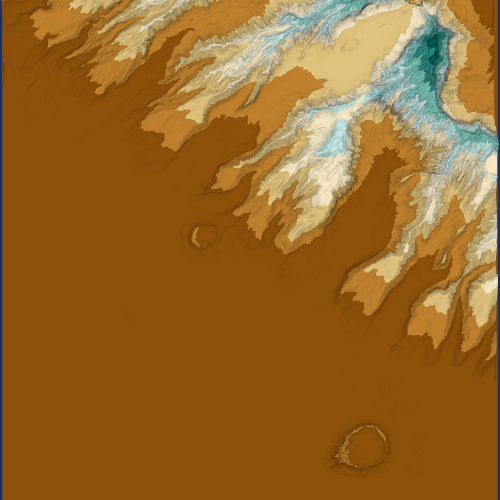
\includegraphics[width=\linewidth]{Figure6-12b}
	\end{subfigure}
	\hfill
	\begin{subfigure}[h]{0.48\linewidth}
		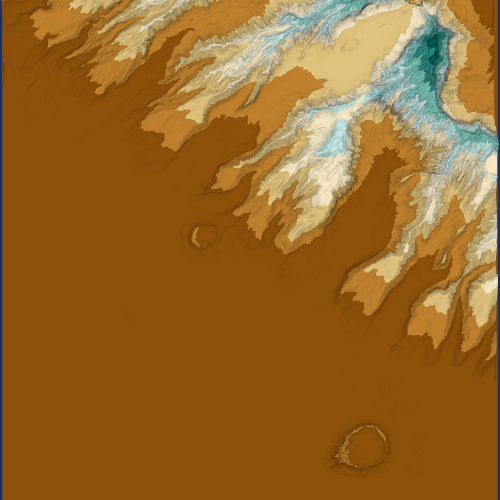
\includegraphics[width=\linewidth]{Figure6-12c}
		\caption*{Applying the technique to terrain data from Honolulu, Hawaii.(\href{https://lorensen.github.io/VTKExamples/site/Cxx/Visualization/Hawaii}{Hawaii.cxx} or \href{https://lorensen.github.io/VTKExamples/site/Python/Visualization/Hawaii/}{Hawaii.py})}
	\end{subfigure}%
	\caption{Computing scalars using normalized dot product.}\label{fig:Figure6-12}
\end{figure}

Part of the creative practice of visualization is selecting the best technique for given data from the palette of available techniques. Often this requires creative mapping by the user of the visualization system. In particular, to use scalar visualization techniques we need only to create a relationship to generate a unique scalar value. Other examples of scalar mapping include an index value into a list of data, computing vector magnitude or matrix determinate, evaluating surface curvature, or determining distance between points. Scalar generation, when coupled with color mapping or contouring, is a simple, yet effective, technique for visualizing many types of data.
\index{algorithms!scalar|)}

\section{Vector Algorithms}
\index{algorithms!vector|(}

Vector data is a three--dimensional representation of direction and magnitude. Vector data often results from the study of fluid flow, or when examining derivatives (i.e., rate of change) of some quantity.

\subsection{Hedgehogs and Oriented Glyphs}
\label{subsec:hedgehogs_oriented_glyphs}
\index{hedgehog|(}

A natural vector visualization technique is to draw an oriented,
scaled line for each vector (Figure \ref{fig:Figure6-13a}). The line begins at the point with which the vector is associated and is oriented in the direction of the vector components $(v_x, v_y, v_z)$. Typically, the resulting line must be scaled up or down to control the size of its visual representation. This technique is often referred to as a \emph{hedgehog} because of the bristly result.

There are many variations of this technique Figure \ref{fig:Figure6-13b}). Arrows may be added to indicate the direction of the line. The lines may be colored according to vector magnitude, or some other scalar quantity (e.g., pressure or temperature). Also, instead of using a line, oriented ``glyphs'' can be used. By glyph we mean any 2D or 3D geometric representation such as an oriented triangle or cone.

\begin{figure}[htb]
	\begin{subfigure}[h]{0.24\linewidth}
		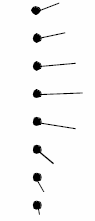
\includegraphics[width=\linewidth]{Figure6-13a}
		\caption{Oriented lines.}\label{fig:Figure6-13a}
	\end{subfigure}
	\hfill
	\begin{subfigure}[h]{0.24\linewidth}
		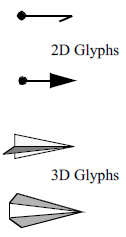
\includegraphics[width=\linewidth]{Figure6-13b}
		\caption{Glyphs}\label{fig:Figure6-13b}
	\end{subfigure}%
	\hfill
	\begin{subfigure}[h]{0.48\linewidth}
		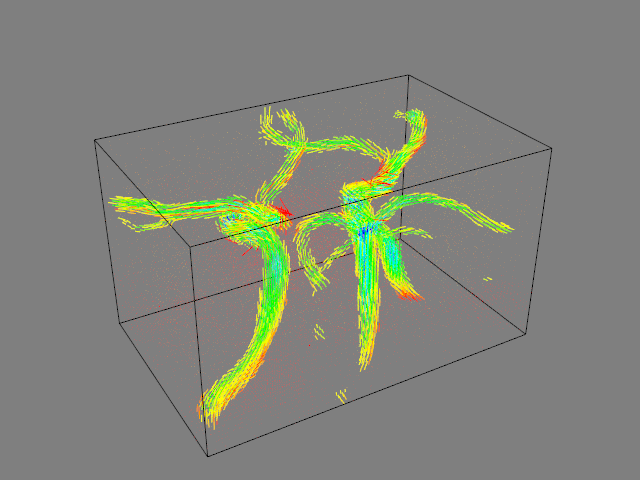
\includegraphics[width=\linewidth]{Figure6-13c}
		\caption{Complex vector visualization. (\href{https://lorensen.github.io/VTKExamples/site/Cxx/Visualization/TestComplexV}{TestComplexV.cxx} or \href{https://lorensen.github.io/VTKExamples/site/Python/Visualization/TestComplexV/}{TestComplexV.py})}\label{fig:Figure6-13c}
	\end{subfigure}
	\caption{Vector visualization techniques.}\label{fig:Figure6-13}
\end{figure}

Care should be used in applying these techniques. In 3D it is often difficult to understand the position and orientation of a vector because of its projection into a 2D image. Also, using large numbers of vectors can clutter the display to the point where the visualization becomes meaningless. Figure \ref{fig:Figure6-13c} shows 167,000 3D vectors (using oriented and scaled lines) in the region of the human carotid artery. The larger vectors lie inside the arteries, the smaller vectors lie outside the arteries and are randomly oriented (measurement error) but small in magnitude. Clearly the details of the vector field are not discernible from this image.

Scaling glyphs also poses interesting problems. In what Tufte has termed a ``visualization lie'', \cite{Tufte83} scaling a 2D or 3D glyph results in nonlinear differences in appearance. The surface area of an object increases with the square of its scale factor, so two vectors differing by a factor of two in magnitude may appear up to four times different based on surface area. Such scaling issues are common in data visualization, and great care must be taken to avoiding misleading viewers.
\index{hedgehog|)}

\subsection{Warping}

Vector data is often associated with ``motion''. The motion is in the form of velocity or displacement. An effective technique for displaying such vector data is to ``warp'' or deform geometry according to the vector field. For example, imagine representing the displacement of a structure under load by deforming the structure. Or if we are visualizing the flow of fluid, we can create a flow profile by distorting a straight line inserted perpendicular to the flow.

\begin{figure}[htb]
	\begin{subfigure}[h]{0.48\linewidth}
	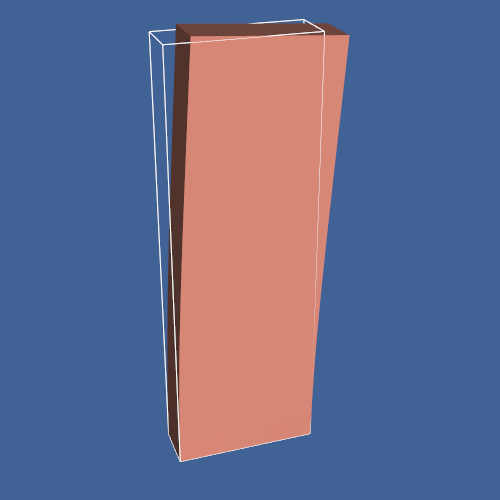
\includegraphics[width=\linewidth]{Figure6-14a}
	\caption{Vibration of beam. (\href{https://lorensen.github.io/VTKExamples/site/Cxx/VisualizationAlgorithms/PlateVibration}{PlateVibration.cxx} or \href{https://lorensen.github.io/VTKExamples/site/Python/VisualizationAlgorithms/PlateVibration/}{PlateVibration.py})}\label{fig:Figure6-14a}
\end{subfigure}
	\hfill
	\begin{subfigure}[h]{0.48\linewidth}
		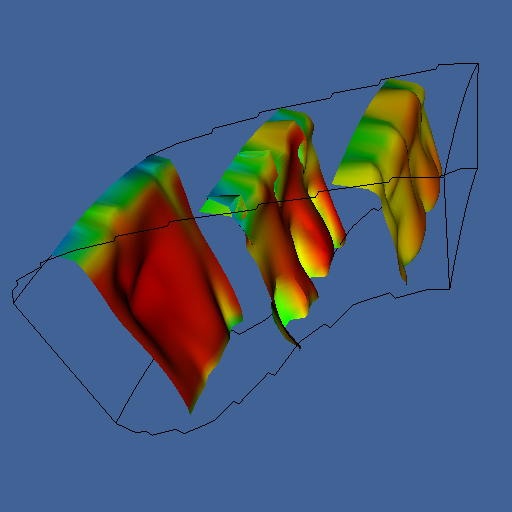
\includegraphics[width=\linewidth]{Figure6-14b}
		\caption{Momentum profiles. (\href{https://lorensen.github.io/VTKExamples/site/Cxx/VisualizationAlgorithms/VelocityProfile}{VelocityProfile.cxx} or \href{https://lorensen.github.io/VTKExamples/site/Python/VisualizationAlgorithms/VelocityProfile/}{VelocityProfile.py})}\label{fig:Figure6-14b}
	\end{subfigure}
	\caption{Warping geometry to show vector field.}\label{fig:Figure6-14}
\end{figure}

Figure \ref{fig:Figure6-14} shows two examples of vector warping. In the first example the motion of a vibrating beam is shown. The original undeformed outline is shown in wireframe. The second example shows warped planes in a structured grid dataset. The planes are warped according to flow momentum. The relative back and forward flow are clearly visible in the deformation of the planes.

Typically, we must scale the vector field to control geometric distortion. Too small a distortion may not be visible, while too large a distortion can cause the structure to turn inside out or selfintersect. In such a case the viewer of the visualization is likely to lose context, and the visualization will become ineffective.

\subsection{Displacement Plots}
\label{subsec:displacement_plots}
\index{displacement plot|(}

Vector displacement on the surface of an object can be visualized with displacement plots. A displacement plot shows the motion of an object in the direction perpendicular to its surface. The object motion is caused by an applied vector field. In a typical application the vector field is a displacement or strain field.

Vector displacement plots draw on the ideas in ``Scalar Generation'' on  page \pageref{subsec:scalar_generation}. Vectors are converted to scalars by computing the dot product between the surface normal and vector at each point (Figure \ref{fig:Figure6-15a}). If positive values result, the motion at the point is in the direction of the surface normal (i.e., positive displacement). Negative values indicate that the motion is opposite the surface normal (i.e., negative displacement).

A useful application of this technique is the study of vibration. In vibration analysis, we are interested in the eigenvalues\index{eigenvalue} (i.e., natural resonant frequencies) and eigenvectors\index{eigenvector} (i.e., mode shapes) of a structure. To understand mode shapes we can use displacement plots to indicate regions of motion. There are special regions in the structure where positive displacement changes to negative displacement. These are regions of zero displacement. When plotted on the surface of the structure, these regions appear as the so-called \emph{modal} lines of vibration. The study of modal lines has long been an important visualization tool for understanding mode shapes.

\begin{figure}[htb]
	\begin{subfigure}[h]{0.48\linewidth}
		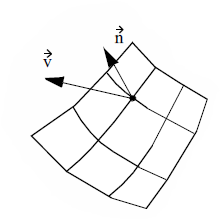
\includegraphics[width=\linewidth]{Figure6-15a}
		\caption{Scalar computation $S = \overrightarrow{v\ } \cdot \overrightarrow{n\ }$.}\label{fig:Figure6-15a}
	\end{subfigure}
	\hfill
	\begin{subfigure}[h]{0.48\linewidth}
		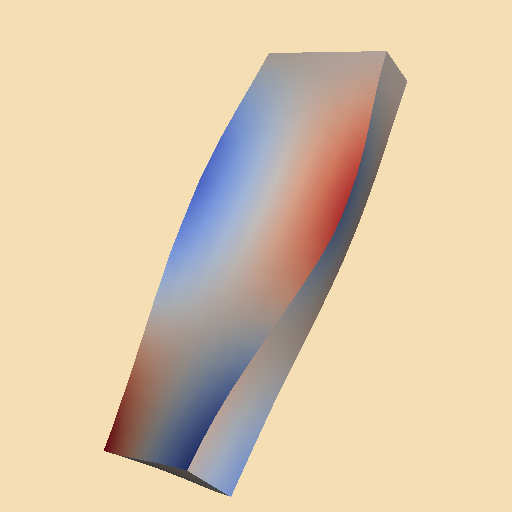
\includegraphics[width=\linewidth]{Figure6-15b}
		\caption{Displacement plot. (\href{https://lorensen.github.io/VTKExamples/site/Cxx/VisualizationAlgorithms/DisplacementPlot}{DisplacementPlot.cxx} or \href{https://lorensen.github.io/VTKExamples/site/Python/VisualizationAlgorithms/DisplacementPlot/}{DisplacementPlot.py})}\label{fig:Figure6-15b}
	\end{subfigure}
	\caption{Vector displacement plots. (a) Vector converted to scalar via dot product computation; (b) Surface plot of vibrating plate. Dark areas show nodal lines. Bright areas show maximum motion.}\label{fig:Figure6-15}
\end{figure}

Figure \ref{fig:Figure6-15b}  shows modal lines for a vibrating rectangular beam. The vibration mode in this figure is the second torsional mode, clearly indicated by the crossing modal lines. (The aliasing in the figure is because of the coarseness of the analysis mesh.) To create the figure we combined the procedure of Figure \ref{fig:Figure6-15a}  with a special lookup table. The lookup table was arranged with white areas in the center (i.e., corresponds to zero dot product) and dark areas at the beginning and end of the table (corresponds to $1$ or $-1$ dot product). As a result, regions of large normal displacement are dark and regions near the modal lines are light.
\index{displacement plot|)}

\subsection{Time Animation}
Some of the techniques described so far can be thought of as moving a point or object over a small time step. The hedgehog line is an approximation of a point's motion over a time period whose duration is given by the scale factor. In other words, if velocity $\vec{V} = dx/dt$, then displacement of a point is

\begin{equation}\label{eq:6.1}
dx = \overrightarrow{V\ }dt
\end{equation}
\myequations{Displacement of a point with respect to time. }

This suggests an extension to our previous techniques: repeatedly displace points over many time steps. Figure \ref{fig:Figure6-16} shows such an approach. Beginning with a sphere \emph{S} centered about some point \emph{C}, we move \emph{S} repeatedly to generate the bubbles shown. The eye tends to trace out a path by connecting the bubbles, giving the observer a qualitative understanding of the fluid flow in that area. The bubbles may be displayed as an animation over time (giving the illusion of motion) or as a multiple exposure sequence (giving the appearance of a path).

\begin{figure}[htb]
	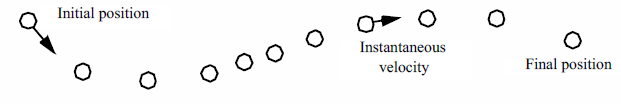
\includegraphics[width=0.96\linewidth]{Figure6-16}
	\caption{Time animation of a point \emph{C}. Although the spacing between points varies, the time increment between each point is constant.}\label{fig:Figure6-16}
\end{figure}

Such an approach can be misused. For one thing, the velocity at a point is instantaneous.

Once we move away from the point the velocity is likely to change. Using Equation \ref{eq:6.1} assumes that the velocity is constant over the entire step. By taking large steps we are likely to jump over changes in the velocity. Using smaller steps we will end in a different position. Thus the choice of step size is a critical parameter in constructing accurate visualization of particle paths in a vector field.

To evaluate Equation \ref{eq:6.1} we can express it as an integral:

\begin{equation}\label{eq:6.2}
\overrightarrow{x\ }(t) = \bigintssss_{t}\overrightarrow{V\ }dt
\end{equation}
\myequations{Integrating velocity with respect to time. }

Although this form cannot be solved analytically for most real world data, its solution can be approximated using numerical integration techniques. Accurate numerical integration is a topic beyond the scope of this book, but it is known that the accuracy of the integration is a function of the step size \emph{$dt$}. Since the path is an integration throughout the dataset, the accuracy of the cell interpolation functions, as well as the accuracy of the original vector data, plays an important role in realizing accurate solutions. No definitive study is yet available that relates cell size or interpolation function characteristics to visualization error. But the lesson is clear: the result of numerical integration must be examined carefully, especially in regions of large vector field gradient. However, as with many other visualization algorithms, the insight gained by using vector integration techniques is qualitatively beneficial, despite the unavoidable numerical errors.

The simplest form of numerical integration is Euler's method,

\begin{equation}\label{eq:6.3}
\overrightarrow{x\ }_{i+1} = \overrightarrow{x\ }_i + \overrightarrow{V\ }_i \Delta{t}
\end{equation}
\myequations{Euler's method. }

where the position at time is the $\overrightarrow{x\ }_{i+1}$ vector sum of the previous position plus the instantaneous velocity times the incremental time step $\Delta{t}$.

Euler's method has error on the order of $O(\Delta{t}^2)$, which is not accurate enough for some applications. One such example is shown in Figure \ref{fig:Figure6-17}. The velocity field describes perfect rotation about a central point. Using Euler's method we find that we will always diverge and, instead of generating circles, will generate spirals instead.

\begin{figure}[htb]
	\begin{subfigure}[h]{0.32\linewidth}
		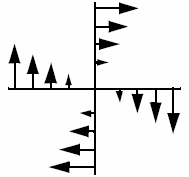
\includegraphics[width=\linewidth]{Figure6-17a}
		\caption{Rotational vector field.}\label{fig:Figure6-17a}
	\end{subfigure}
	\hfill
	\begin{subfigure}[h]{0.32\linewidth}
	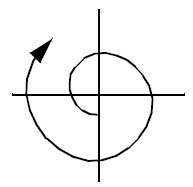
\includegraphics[width=\linewidth]{Figure6-17b}
	\caption{Euler's method.}\label{fig:Figure6-17b}
	\end{subfigure}
	\hfill
	\begin{subfigure}[h]{0.32\linewidth}
	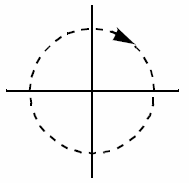
\includegraphics[width=\linewidth]{Figure6-17c}
	\caption{Runge-Kutta..}\label{fig:Figure6-17c}
\end{subfigure}
	\caption{Euler's integration (b) and Runge-Kutta integration of order 2 (c) applied to uniform rotational vector field (a). Euler's method will always diverge.}\label{fig:Figure6-17}
\end{figure}

In this text we will use the Runge--Kutta technique of order $2$ \cite{Conte72}. This is given by the expression

\begin{equation}\label{eq:6.4}
\overrightarrow{x\ }_{i+1} = \overrightarrow{x\ }_i +\frac{\Delta t}{2}(\overrightarrow{V\ }_i + \overrightarrow{V\ }_{i+1})
\end{equation}
\myequations{Runge--Kutta technique of order $2$. }

One final note about accuracy concerns. The errors involved in either perception or computation of visualizations is an open research area. The discussion in the preceding paragraph is a good example of this. There we characterized the error in streamline integration using conventional numerical integration arguments. But there is a problem with this argument. In visualization applications, we are integrating across cells whose function values are continuous, but whose derivatives are not. As the streamline crosses the cell boundary, subtle effects may occur that are not treated by the standard numerical analysis. Thus the standard arguments need to be extended for visualization applications.

Integration formulas require repeated transformation from global to local coordinates. Consider moving a point through a dataset under the influence of a vector field. The first step is to identify the cell that contains the point. This operation is a search (see ``Searching'' on page \pageref{sec:searching} ), plus a conversion to local coordinates. Once the cell is found, then the next step is to compute the velocity at that point by interpolating the velocity from the cell points. The point is then incrementally repositioned (using the integration formula Equation \ref{eq:6.4}).
The process is then repeated until the point exits the dataset or the distance or time traversed exceeds some specified value.

This process can be computationally demanding. There are two important steps we can take to improve performance.

\begin{enumerate}

\item \emph{Improving search procedures.} There are two distinct types of searches. Initially, the starting location of the particle must be determined by a global search procedure. Once the initial location of the point is determined in the dataset, an incremental search procedure can then be used. Incremental searching is efficient because the motion of the point is limited within a single cell, or at most across a cell boundary. Thus, the search space is greatly limited, and the incremental search is faster relative to the global search.

\item \emph{Coordinate transformation.} The cost of a coordinate transformation from global to local coordinates can be reduced if either of the following conditions are true: the local and global coordinate systems are identical with one another (or vary by \emph{xyz} translation), or if the vector field is transformed from global space to local coordinate space. The image data coordinate system is an example of a local coordinates which are parallel to global coordinates, hence global to local coordinate transformation can be greatly accelerated. If the vector field is transformed into local coordinates (either as a preprocessing step or on a cell by cell basis), then the integration can proceed completely in local space. Once the integration path is computed, selected points along the path can be transformed into global space for the sake of visualization.

\end{enumerate}

\subsection{Streamlines}

A natural extension of the previous time animation techniques is to connect the point position over many time steps. The result is a numerical approximation to a particle trace represented as a line.

Borrowing terminology from the study of fluid flow, we can define three related line representation schemes for vector fields.

\begin{itemize}

\item \emph{Particle traces} are trajectories traced by fluid particles over time.

\item \emph{Streaklines} are the set of particle traces at a particular time $t_i$ through a specified point $x_i$.

\item \emph{Streamlines} are integral curves along a curve $s$ satisfying the equation

\begin{equation}\label{eq:6.5}
s = \bigintssss_{t}\overrightarrow{V\ }ds, \ \text{with}\ s = (x,t)
\end{equation}
\myequations{Streamline.}
for a particular time $t$.
\end{itemize}

Streamlines, streaklines, and particle traces are equivalent to one another if the flow is steady. In time--varying flow, a given streamline exists only at one moment in time. Visualization systems generally provide facilities to compute particle traces. However, if time is fixed, the same facility can be used to compute streamlines. In general, we will use the term streamline to refer to the method of tracing trajectories in a vector field. Please bear in mind the differences in these representations if the flow is time--varying.

Figure \ref{fig:Figure6-18} shows forty streamlines in a small kitchen. The room has two windows, a door (with air leakage), and a cooking area with a hot stove. The air leakage and temperature variation combine to produce air convection currents throughout the kitchen. The starting positions of the streamlines were defined by creating a \emph{rake}, or curve (and its associated points). Here the rake was a straight line. These streamlines clearly show features of the flow field. By releasing many streamlines simultaneously we obtain even more information, as the eye tends to assemble nearby streamlines into a ``global'' understanding of flow field features.

\begin{figure}[htb]
	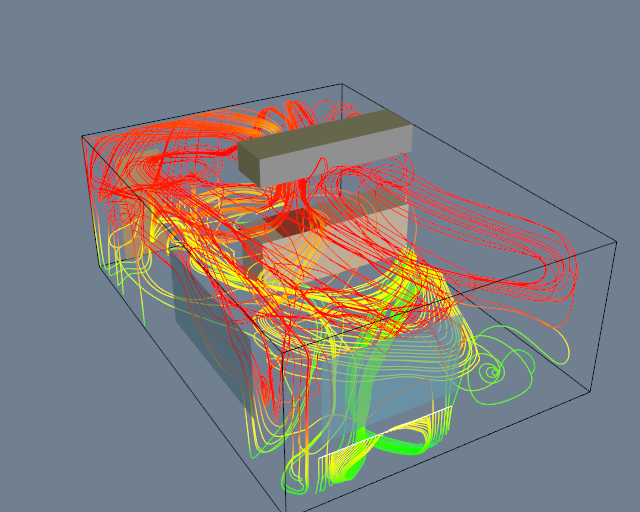
\includegraphics[width=0.96\linewidth]{Figure6-18}
	\caption{Flow velocity computed for a small kitchen. Forty streamlines start along the rake positioned under the window. Some eventually travel over the hot stove and are convected upwards. (\href{https://lorensen.github.io/VTKExamples/site/Cxx/Visualization/Kitchen}{Kitchen.cxx} or \href{https://lorensen.github.io/VTKExamples/site/Python/Visualization/Kitchen/}{Kitchen.py})}\label{fig:Figure6-18}
\end{figure}

Many enhancements of streamline visualization exist. Lines can be colored according to velocity magnitude to indicate speed of flow. Other scalar quantities such as temperature or pressure also may be used to color the lines. We also may create constant time dashed lines. Each dash represents a constant time increment. Thus, in areas of high velocity, the length of the dash will be greater relative to regions of lower velocity. These techniques are illustrated in Figure \ref{fig:Figure6-19} for airflow around a blunt fin. This example consists of a wall with half a rounded fin projecting into the fluid flow. (Using arguments of symmetry, only half of the domain was modeled.) Twenty five streamlines are released upstream of the fin. The boundary layer effects near the junction of the fin and wall are clearly evident from the streamlines. In this area, flow recirculation is apparent, as well as the reduced flow speed.

\begin{figure}[htb]
	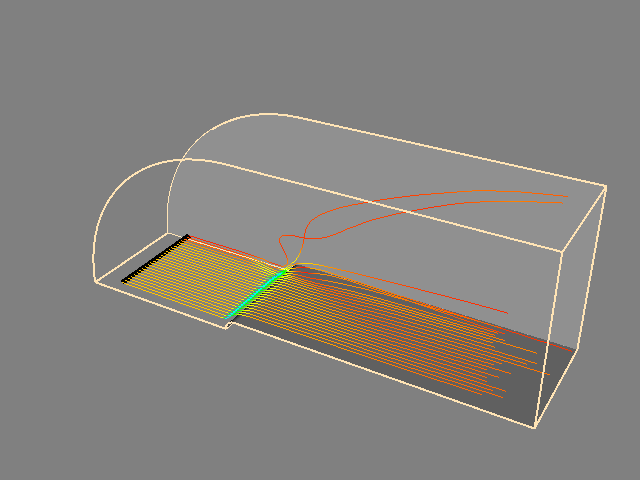
\includegraphics[width=0.96\linewidth]{Figure6-19}
	\caption{airflow around a blunt fin. (\href{https://lorensen.github.io/VTKExamples/site/Cxx/VisualizationAlgorithms/BluntStreamlines}{BluntStreamlines.cxx} or \href{https://lorensen.github.io/VTKExamples/site/Python/VisualizationAlgorithms/BluntStreamlines/}{BluntStreamlines.py})}\label{fig:Figure6-19}
\end{figure}

\index{algorithms!vector|)}

\section{Tensor Algorithms}
\index{algorithms!tensor|(}

As we mentioned earlier, tensor visualization is an active area of research. However there are a few simple techniques that we can use to visualize real $3 \times 3$ symmetric tensors. Such tensors are used to describe the state of displacement or stress in a 3D material. The stress and strain tensors for an elastic material are shown in Figure \ref{fig:Figure6-20}.

In these tensors the diagonal coefficients are the so--called normal stresses and strains, and the off-diagonal terms are the shear stresses and strains. Normal stresses and strains act perpendicular to a specified surface, while shear stresses and strains act tangentially to the surface. Normal stress is either compression or tension, depending on the sign of the coefficient.

A $3 \times 3$ real symmetric matrix can be characterized by three vectors in 3D called the eigenvectors\index{eigenvector}, and three numbers called the eigenvalues\index{eigenvalue} of the matrix. The eigenvectors form a 3D coordinate system whose axes are mutually perpendicular. In some applications, particularly the study of materials, these axes also are referred to as the principle axes of the tensor and are physically significant. For example, if the tensor is a stress tensor, then the principle axes are the directions of normal stress and no shear stress. Associated with each eigenvector is an eigenvalue. The eigenvalues are often physically significant as well. In the study of vibration, eigenvalues correspond to the resonant frequencies of a structure, and the eigenvectors are the associated mode shapes.

Mathematically we can represent eigenvalues and eigenvectors as follows. Given a matrix $A$ the eigenvector $\overrightarrow{x\ }$ and eigenvalue $\lambda$ must satisfy the relation 

\begin{equation}\label{eq:6.6}
A \cdot x = \lambda\ \  \overrightarrow{x\ }
\end{equation}
\myequations{Relation between eigenvalues and eigenvectors.}

\noindent For Equation \ref{eq:6.6} to hold, the matrix determinant must satisfy

\begin{equation}\label{eq:6.7}
det |A-\lambda I| = 0
\end{equation}
\myequations{Condition for Equation \ref{eq:6.6} to hold.}

\noindent Expanding this equation yields a $n^{th}$ degree polynomial in $\lambda$ whose roots are the eigenvalues. Thus, there are always $n$ eigenvalues, although they may not be distinct. In general, Equation \ref{eq:6.7} is not solved using polynomial root searching because of poor computational performance. (For matrices of order 3 root searching is acceptable because we can solve for the eigenvalues analytically.) Once we determine the eigenvalues, we can substitute each into Equation \ref{eq:6.7} to solve for the associated eigenvectors.


\begin{figure}[htb]
	\begin{subfigure}[h]{0.48\linewidth}
		\Large
		\begin{equation*}
		\left[\begin{array}{ccc}
		\sigma{_x} & \tau{_{xy}} & \tau{_{xz}}  \\
		\tau{_{yx}} & \sigma{_y} & \tau{_{yz}}    \\
		\tau{_{zx}} & \tau{_{zy}} & \sigma{_z}
		\end{array}\right]
		\end{equation*}
		\caption{Stress tensor.}
		\label{fig:Figure6-20a}
	\end{subfigure}
	\hfill
	\begin{subfigure}[h]{0.48\linewidth}
		\Large
		\begin{equation*}
		\left[\begin{array}{ccc}
		\frac{\partial u}{\partial x} & (\frac{\partial u}{\partial y} + \frac{\partial v}{\partial z})&   (\frac{\partial u}{\partial z} + \frac{\partial w}{\partial x})\\ \\
		(\frac{\partial u}{\partial y} + \frac{\partial v}{\partial z}) & \frac{\partial v}{\partial y} & (\frac{\partial v}{\partial z} + \frac{\partial w}{\partial y})    \\ \\
		(\frac{\partial u}{\partial z} + \frac{\partial w}{\partial x}) & (\frac{\partial v}{\partial z} + \frac{\partial w}{\partial y})&
		\frac{\partial w}{\partial z}
		\end{array}\right]
		\end{equation*}
		\caption{Strain tensor}\label{fig:Figure6-20b}
	\end{subfigure}
	\caption{Stress and strain tensors. Normal stresses in the $x-y-z$ coordinate directions indicated as $(\sigma_x, \sigma_y, \sigma_z)$, shear stresses indicated as $t_{ij}$. Material displacement represented by $(u, v, w)$ components.}\label{fig:Figure6-20}
\end{figure}


We can express the eigenvectors of the $3 \times 3$ system as

\begin{equation}\label{eq:6.8}
\vec{v_i} = \lambda _i \vec{e_i} \ with\  i = 1,2,3
\end{equation}
\myequations{Eigenvectors of the  $3 \times 3$ system.}

with $\vec{e_i}$ a unit vector in the direction of the eigenvalue, and $\lambda{_i}$ the eigenvalues of the system. If we order eigenvalues such that

\begin{equation}\label{eq:6.9}
\lambda{_1} \geq \lambda{_2} \geq \lambda{_3}
\end{equation}
\myequations{Ordering of eigenvalues.}

then we refer to the corresponding eigenvectors $\vec{v_1}$, $\vec{v_2}$ and $\vec{v_1}$ as the \emph{major}, \emph{medium} and \emph{minor} eigenvectors.

\subsection{Tensor Ellipsoids}

This leads us to the tensor ellipsoid technique for the visualization of real, symmetric $3 \times 3$ matrices. The first step is to extract eigenvalues and eigenvectors as described in the previous section. Since eigenvectors are known to be orthogonal, the eigenvectors form a local coordinate system. These axes can be taken as the \emph{minor}, \emph{medium} and \emph{major} axes of an ellipsoid. Thus, the shape and orientation of the ellipsoid represents the relative size of the eigenvalues and the orientation of the eigenvectors.

To form the ellipsoid we begin by positioning a sphere at the tensor location. The sphere is then rotated around its origin using the eigenvectors, which in the form of Equation \ref{eq:6.8} are direction cosines. The eigenvalues are used to scale the sphere. Using $4 \times 4$ transformation matrices and referring to Equation \ref{eq:3.6}, Equation \ref{eq:3.9} and Equation \ref{eq:3.13}, we form the ellipsoid by transforming the sphere centered at the origin using the matrix $T$

\begin{equation}\label{eq:6.10}
T = T_T \cdot T_R \cdot T_S
\end{equation}
\myequations{Transforming the sphere.}

(remember to read right to left). The eigenvectors can be directly plugged in to create the rotation matrix, while the point coordinates $x-y-z$ and eigenvalues $\lambda{_1} \geq \lambda{_2} \geq \lambda{_3}$ are inserted into the translation and scaling matrices. A concatenation of these matrices forms the final transformation matrix $T$.


\begin{figure}[htb]
	\begin{subfigure}[h]{0.48\linewidth}
		%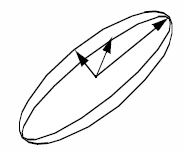
\includegraphics[width=0.96\linewidth]{Figure6-21a}
		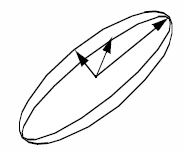
\includegraphics{Figure6-21a}
		\caption{Tensor ellipsoid.}
		\label{fig:Figure6-21a}
	\end{subfigure}
	\hfill
	\begin{subfigure}[h]{0.48\linewidth}
		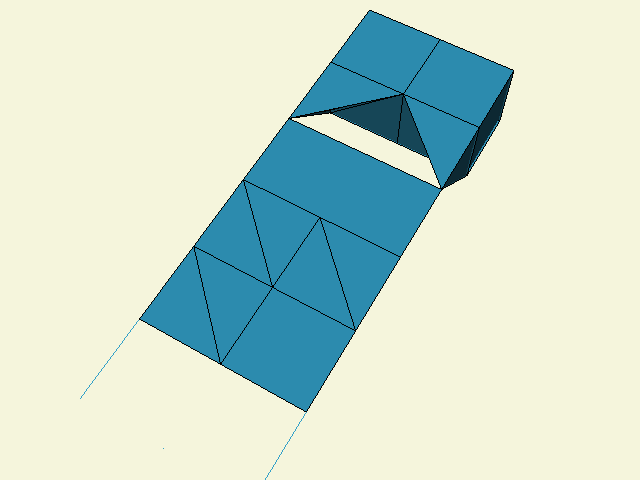
\includegraphics[width=0.96\linewidth]{Figure6-21b}
		\caption{Point load on semifinite domain.}
		\label{fig:Figure6-21b}
	\end{subfigure}
	\hfill
	\begin{subfigure}[h]{0.96\linewidth}
		\Large
		\begin{equation*}
		\begin{array}{l}
				\begin{array}{lll}
				\sigma{_x} & = &  -\frac{P}{2 \pi \rho ^2}\left(\frac{3zx^2}{\rho ^3} -(1-2v)\left((\frac{z}{\rho\
				} - \frac{\rho}{\rho+z}+\frac{x ^2 (2 \rho + z)}{\rho ( \rho + z) ^2} \right) \right)\\
				\sigma{_y}  & = & -\frac{P}{2 \pi \rho ^2}\left(\frac{3zy^2}{\rho ^3} -(1-2v)\left((\frac{z}{\rho\
				} - \frac{\rho}{\rho+z}+\frac{y ^2 (2 \rho + z)}{\rho ( \rho + z) ^2} \right) \right)  \\
			    \sigma{_z}  & = & \frac{3Pz^3}{2\pi\rho^5}
				\end{array} \\
				\begin{array}{lllll}
				\tau_{xy} &=& \tau_{yx} &=& -\frac{P}{2 \pi \rho ^2}\left( \frac{3xyz}{\rho ^3} - (1-2v)\left(\frac{xy(2 \rho + z)}{\rho ( \rho + z) ^2}\right)\right) \\
				\tau_{xz}&=&\tau_{zx} &=& -\frac{3Pxz^2}{2 \pi \rho ^5}\\
				\tau_{yz}&=&\tau_{zy} &=& -\frac{3Pyz^2}{2 \pi \rho ^5}
				\end{array}
		\end{array}
	\end{equation*}
		\caption{Analytic solution}\label{fig:Figure6-21c}
	\end{subfigure}
	\caption{Stress and strain tensors. Normal stresses in the $x-y-z$ coordinate directions indicated as $(\sigma_x, \sigma_y, \sigma_z)$, shear stresses indicated as $t_{ij}$. Material displacement represented by $(u, v, w)$ components.}\label{fig:Figure6-21}
\end{figure}

Figure \ref{fig:Figure6-21a} depicts the tensor ellipsoid technique. In Figure \ref{fig:Figure6-21b}) we show this technique to visualize material stress near a point load on the surface of a semiinfinite domain. (This is the so-called Boussinesq's problem.) From Saada \cite{Saada74} we have the analytic expression for the stress components in Cartesian coordinates shown in Figure \ref{fig:Figure6-21c}. Note that the $z$-direction is defined as the axis originating at the point of application of the force $P$. The variable $\rho$ is the distance from the point of load application to a point $x-y-z$. The orientation of the $x$ and $y$ axes are in the plane perpendicular to the $z$ axis. (The rotation in the plane of these axes is unimportant since the solution is symmetric around the $z$ axis.) (The parameter $\nu$ is Poisson's ratio which is a property of the material. Poisson's ratio relates the lateral contraction of a material to axial elongation under a uniaxial stress condition. See \cite{Saada74} or \cite{Timoshenko70} for more information.)

\begin{figure}[htb]
	\begin{subfigure}[h]{0.48\linewidth}
		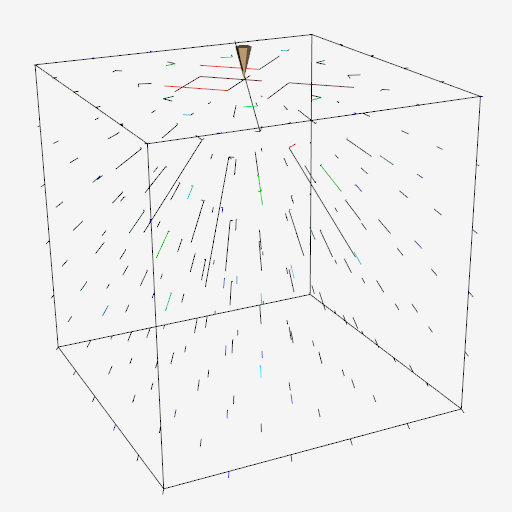
\includegraphics[width=0.96\linewidth]{Figure6-22a}
		\caption{Tensor axes. (\href{https://lorensen.github.io/VTKExamples/site/Cxx/VisualizationAlgorithms/TensorAxes}{TensorAxes.cxx} or \href{https://lorensen.github.io/VTKExamples/site/Python/VisualizationAlgorithms/TensorAxes/}{TensorAxes.py})}
		\label{fig:Figure6-22a}
	\end{subfigure}
	\hfill
	\begin{subfigure}[h]{0.48\linewidth}
		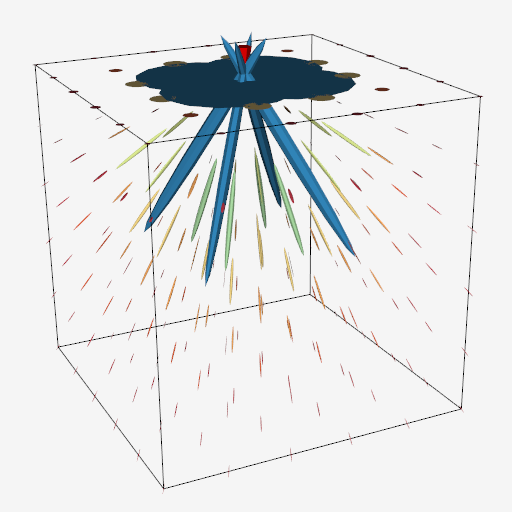
\includegraphics[width=0.96\linewidth]{Figure6-22b}
		\caption{Tensor ellipsiods. (\href{https://lorensen.github.io/VTKExamples/site/Cxx/VisualizationAlgorithms/TensorEllipsoids}{TensorEllipsoids.cxx} or \href{https://lorensen.github.io/VTKExamples/site/Python/VisualizationAlgorithms/TensorEllipsoids/}{TensorEllipsoids.py})}
		\label{fig:Figure6-22b}
	\end{subfigure}
	\caption{Tensor visualization techniques; (a) Tensor axes, (b) Tensor ellipsiods.}\label{fig:Figure6-22}
\end{figure}

In Figure \ref{fig:Figure6-21a} we visualize the analytical results of Boussinesq's problem from Saada. The top portion of the figure shows the results by displaying the scaled and oriented principal axes of the stress tensor. (These are called \emph{tensor axes}.) In the bottom portion we use tensor ellipsoids to show the same result. Tensor ellipsoids and tensor axes are a form of \emph{glyph} (see "Glyphs" on page \pageref{subsec:glyphs} ) specialized to tensor visualization.

A certain amount of care must be taken to visualize this result since there is a stress singularity at the point of contact of the load. In a real application loads are applied over a small area and not at a single point. Also, plastic behavior prevents stress levels from exceeding a certain point. The results of the visualization, as with any computer process, are only as good as the underlying model.
\index{algorithms!tensor|)}

\section{Modelling Algorithms}
\index{algorithms!modelling|(}

Modelling algorithms are the catchall category for our taxonomy of visualization techniques. Modelling algorithms have one thing in common: They create or change dataset geometry or topology.

\subsection{Source Objects}

As we have seen in previous examples, source objects begin the visualization pipeline. Source objects are used to create geometry such as spheres, cones, or cubes to support visualization context or are used to read in data files. Source objects also may be used to create dataset attributes. Some examples of source objects and their use are as follows.

\begin{description}[leftmargin=0cm,labelindent=0cm]

\item[Modelling Simple Geometry.] Spheres, cones, cubes, and other simple geometric objects can be used alone or in combination to model geometry. Often we visualize real--world applications such as air flow in a room and need to show real-world objects such as furniture, windows, or doors.
Real--world objects often can be represented using these simple geometric representations. These source objects generate their data procedurally. Alternatively, we may use reader objects to access geometric data defined in data files. These data files may contain more complex geometry such as that produced by a 3D CAD (ComputerAided Design) system.

\item[Supporting Geometry.] During the visualization process we may use source objects to create supporting geometry. This may be as simple as three lines to represent a coordinate axis or as complex as tubes wrapped around line segments to thicken and enhance their appearance. Another common use is as supplemental input to objects such as streamlines or probe filters. These filters take a second input that defines a set of points. For streamlines, the points determine the initial positions for generating the streamlines. The probe filter uses the points as the position to compute attribute values such as scalars, vectors, or tensors.

\item[Data Attribute Creation.] Source objects can be used as procedures to create data attributes. For example, we can procedurally create textures and texture coordinates. Another use is to create scalar values over a uniform grid. If the scalar values are generated from a mathematical function, then we can use the visualization techniques described here to visualize the function. In fact, this leads us to a very important class of source objects: implicit functions.

\end{description}

\subsection{Implicit Functions}
\label{subsec:implicit_functions}
\index{implicit function|(}

Implicit functions are functions of the form

\begin{equation}\label{eq:6.11}
F(x,y,z) = c
\end{equation}
\myequations{Implicit function.}

where $c$ is an arbitrary constant. Implicit functions have three
important properties.

\begin{itemize}

\item \emph{Simple geometric description.} Implicit functions are convenient tools to describe common geometric shapes. This includes planes, spheres, cylinders, cones, ellipsoids, and quadrics.

\item \emph{Region separation.} Implicit functions separate 3D Euclidean space into three distinct regions. These regions are inside, on, and outside the implicit function. These regions are defined as $F(x,y,z) < 0$, $F(x,y,z) = 0$ and $F(x,y,z) > 0$, respectively.

\item \emph{Scalar generation.} Implicit functions convert a position in space into a scalar value. That is, given an implicit function we can sample it at a point $(x_i,y_i,z_i)$ to generate a scalar value $c_i$.

\end{itemize}

An example of an implicit function is the equation for a sphere of radius $R$.

\begin{equation}\label{eq:6.12}
F(x,y,z) = x^2 + y^2 + z^2 - R^2
\end{equation}
\myequations{Implicit function for a sphere.}

This simple relationship defines the three regions (on $F(x,y,z = 0)$ on the sphere), $F(x,y,z) < 0$ (inside the sphere), and $F(x,y,z) > 0$ (outside the sphere). Any point maybe be classified as inside, on, or outside the sphere simply by evaluating Equation \ref{eq:6.12}.

\begin{figure}[htb]
	\begin{subfigure}[h]{0.32\linewidth}
		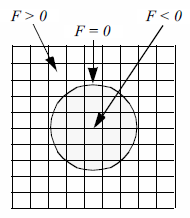
\includegraphics[width=0.96\linewidth]{Figure6-23a}
		\caption{2D depiction of sphere sampling.}
		\label{fig:Figure6-23a}
	\end{subfigure}
	\begin{subfigure}[h]{0.32\linewidth}
		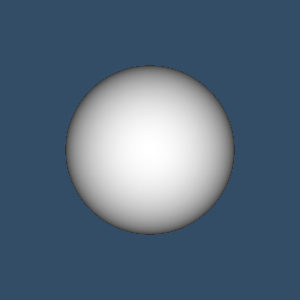
\includegraphics[width=0.96\linewidth]{Figure6-23b}
		\caption{Isosurface of a sphere. (\href{https://lorensen.github.io/VTKExamples/site/Cxx/ImplicitFunctions/ImplicitSphere}{ImplicitSphere.cxx} or \href{https://lorensen.github.io/VTKExamples/site/Python/ImplicitFunctions/ImplicitSphere/}{ImplicitSphere.py})}
		\label{fig:Figure6-23b}
	\end{subfigure}
	\hfill
	\begin{subfigure}[h]{0.32\linewidth}
		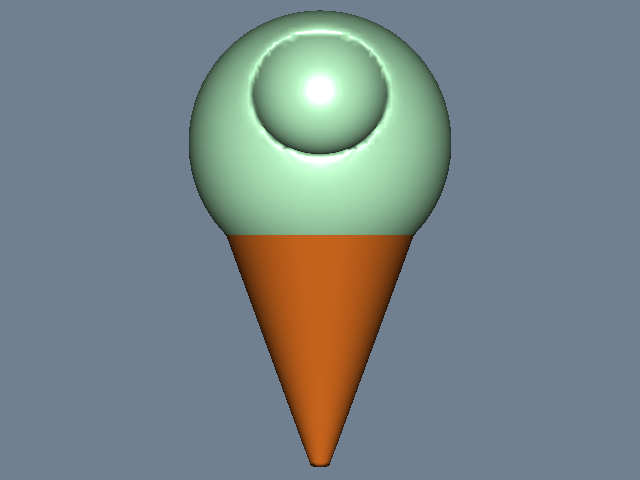
\includegraphics[width=0.96\linewidth]{Figure6-23c}
		\caption{Boolean combination of two spheres. (\href{https://lorensen.github.io/VTKExamples/site/Cxx/VisualizationAlgorithms/IceCream}{IceCream.cxx} or \href{https://lorensen.github.io/VTKExamples/site/Python/VisualizationAlgorithms/IceCream/}{IceCream.py})}
		\label{fig:Figure6-23c}
	\end{subfigure}
	\caption{Sampling functions: (a) 2D depiction of sphere sampling] (b) Isosurface of sampled sphere; (c) Boolean combination of two spheres, a cone, and two planes. (One sphere intersects the other, the planes clip the cone).}\label{fig:Figure6-23}
\end{figure}

Implicit functions have a variety of uses. This includes geometric modelling, selecting data, and visualizing complex mathematical descriptions.
\index{implicit function|)}

\begin{description}[leftmargin=0cm,labelindent=0cm]

\item[Modelling Objects.] Implicit functions can be used alone or in combination to model geometric objects. For example, to model a surface described by an implicit function\index{isosurface}, we sample $F$ on a dataset and generate an isosurface at a contour value $c_i$. The result is a polygonal representation of the function. Figure \ref{fig:Figure6-23b} shows an isosurface for a sphere of radius=1 sampled on a volume. Note that we can choose nonzero contour values to generate a family of offset surfaces. This is useful for creating blending functions and other special effects.

Implicit functions can be combined to create complex objects using the boolean operators\index{boolean operators} union, intersection, and difference. The union operation between $F\cup G$ between two functions $F(x,y,z)$ and $G(x,y,z)$ is the minimum value

\begin{equation}\label{eq:6.13}
F \cup G = \lbrace \max\left(F\left(\overrightarrow{\ x\ }\right), G\left(\overrightarrow{\ x\ }\right)\right)\, \vert \, \overrightarrow{\ x\ } \in \mathbb{R}^n \rbrace
\end{equation}
\myequations{Union.}

The intersection between two implicit functions is given by

\begin{equation}\label{eq:6.14}
F \cap G = \lbrace \min\left(F\left(\overrightarrow{\ x\ }\right), G\left(\overrightarrow{\ x\ }\right)\right)\, \vert \, \overrightarrow{\ x\ } \in \mathbb{R}^n  \rbrace
\end{equation}
\myequations{Intersection.}

The difference of two implicit functions is given by

\begin{equation}\label{eq:6.15}
F - G = \lbrace \min\left(F\left(\overrightarrow{\ x\ }\right), -G\left(\overrightarrow{\ x\ }\right)\right)\, \vert \, \overrightarrow{\ x\ } \in \mathbb{R}^n  \rbrace
\end{equation}
\myequations{Difference.}

Figure \ref{fig:Figure6-23c} shows a combination of simple implicit functions to create an ice-cream cone. The cone is created by clipping the (infinite) cone function with two planes. The ice cream is constructed by performing a difference operation on a larger sphere with a smaller offset sphere to create the ``bite.'' The resulting surface was extracted using surface contouring with isosurface value $0.0$.

\begin{figure}[htb]
	\begin{subfigure}[h]{0.48\linewidth}
		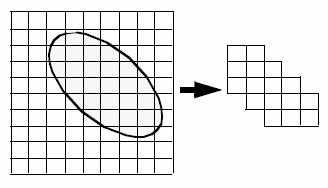
\includegraphics[width=0.96\linewidth]{Figure6-24a}
		\caption{Selecting data with implicit function}
		\label{fig:Figure6-24a}
	\end{subfigure}
	\hfill
	\begin{subfigure}[h]{0.48\linewidth}
		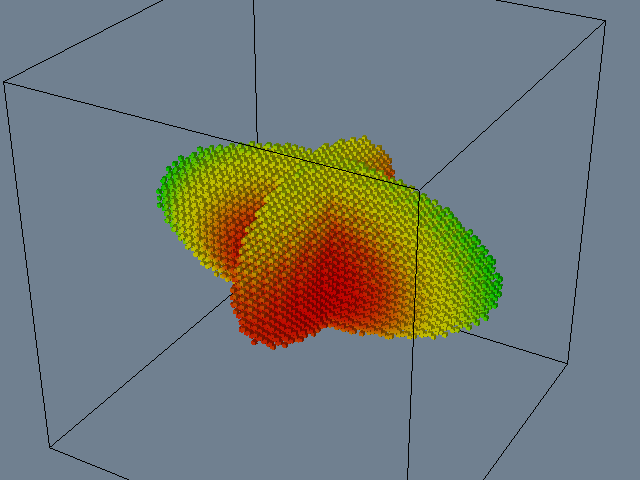
\includegraphics[width=0.96\linewidth]{Figure6-24b}
		\caption{Isosurface of a sphere. (\href{https://lorensen.github.io/VTKExamples/site/Cxx/VisualizationAlgorithms/ExtractData}{ExtractData.cxx} or \href{https://lorensen.github.io/VTKExamples/site/Python/VisualizationAlgorithms/ExtractData/}{ExtractData.py})}
		\label{fig:Figure6-24b}
	\end{subfigure}
	\caption{Implicit functions used to select data: (a) 2D cells lying in ellipse are selected; (b) Two ellipsoids combined using the union operation used to select voxels from a volume. Voxels shrunk 50 percent.}\label{fig:Figure6-24}
\end{figure}

\item[Selecting Data.] We can take advantage of the properties of implicit functions to select and cut data. In particular we will use the region separation property to select data. (We defer the discussion on cutting to "Cutting" on page \pageref{subsec:cutting}.)

Selecting or extracting data with an implicit function means choosing cells and points (and associated attribute data) that lie within a particular region of the function. To determine whether a point \emph{xyz} lies within a region, we simply evaluate the point and examine the sign of the result. A cell lies in a region if all its points lie in the region.

Figure \ref{fig:Figure6-24a} shows a 2D implicit function, here an ellipse, used to select the data (i.e., points, cells, and data attributes) contained within it. Boolean combinations also can be used to create complex selection regions as illustrated in Figure \ref{fig:Figure6-24b}. Here, two ellipses are used in combination to select voxels within a volume dataset. Note that extracting data often changes the structure of the dataset. In Figure \ref{fig:Figure6-24} the input type is a image data dataset, while the output type is an unstructured grid dataset.

\item[Visualizing Mathematical Descriptions.] Some functions, often discrete or probabilistic in nature, cannot be cast into the form of Equation \ref{eq:6.11}. However, by applying some creative thinking we can often generate scalar values that can be visualized. An interesting example of this is the so--called \emph{strange attractor}.

Strange attractors arise in the study of nonlinear dynamics and chaotic systems. In these systems, the usual types of dynamic motion --- equilibrium, periodic motion, or quasiperiodic motion --- are not present. Instead, the system exhibits chaotic motion. The resulting behavior of the system can change radically as a result of small perturbations in its initial conditions.

\begin{figure}[htb]
	\begin{subfigure}[h]{0.48\linewidth}
		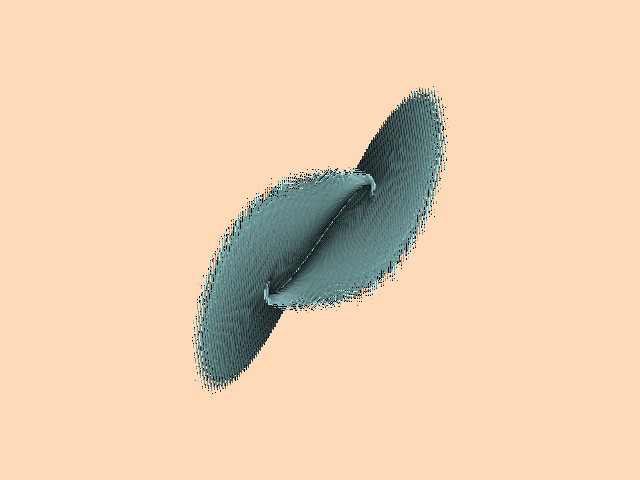
\includegraphics[width=0.96\linewidth]{Figure6-25a}
		\caption{}
		\label{fig:Figure6-25a}
	\end{subfigure}
	\hfill
	\begin{subfigure}[h]{0.48\linewidth}
        % We do not have Figure6-25b so this is the scraped one from the book.
		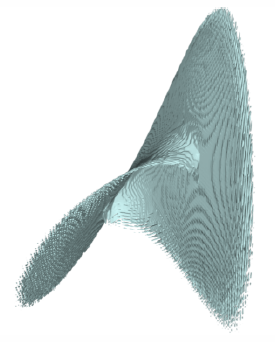
\includegraphics[width=0.96\linewidth]{Figure6-25b}
		\caption{}
		\label{fig:Figure6-25b}
	\end{subfigure}
	\caption{Visualizing a Lorenz strange attractor by integrating the Lorenz equations in a volume. The number of visits in each voxel is recorded as a scalar function. The surface is extracted via marching cubes\index{marching cubes} using a visit value of 50. The number of integration steps is 10 million, in a volume of dimensions $200^3$. The surface roughness is caused by the discrete nature of the evaluation function.(\href{https://lorensen.github.io/VTKExamples/site/Cxx/Visualization/Lorenz}{Lorenz.cxx} or \href{https://lorensen.github.io/VTKExamples/site/Python/Visualization/Lorenz/}{Lorenz.py})}\label{fig:Figure6-25}
\end{figure}

A classical strange attractor was developed by Lorenz in 1963 \cite{Lorenz63}. Lorenz developed a simple model for thermally induced fluid convection in the atmosphere. Convection causes rings of rotating fluid and can be developed from the general Navier Stokes partial differential equations for fluid flow. The Lorenz equations can be expressed in nondimensional form as

\begin{equation}\label{eq:6.16}
\begin{array}{lll}
\dfrac{\text{d}x}{\text{d}t} &=& \sigma (y - z) \\ \\
\dfrac{\text{d}y}{\text{d}t} &=& \rho x - y - x z \\ \\
\dfrac{\text{d}z}{\text{d}t} &=& x y - \beta z
\end{array}
\end{equation}
\myequations{Lorenz equations for Navier Stokes partial differential equations for fluid flow.}

where $x$ is proportional to the fluid velocity in the fluid ring, $y$ and $z$z measure the fluid temperature in the plane of the ring, the parameters $\sigma$ and $\rho$ are related  to the Prandtl number\index{Prandtl number} and Raleigh number\index{Raleigh number}, respectively, and $\beta$ is a geometric factor.

Certainly these equations are not in the implicit form of Equation \ref{eq:6.11}, so how do we visualize them? Our solution is to treat the variables x, y, and z as the coordinates of a three--dimensional space, and integrate Equation \ref{eq:6.16} to generate the system ``trajectory'', that is, the state of the system through time. The integration is carried out within a volume and scalars are created by counting the number of times each voxel is visited. By integrating long enough, we can create a volume representing the ``surface'' of the strange attractor, Figure \ref{fig:Figure6-25}. The surface of the strange attractor is extracted by using marching cubes\index{marching cubes!and strange attractors} and a scalar value specifying the number of visits in a voxel.

\end{description}

\subsection{Implicit Modelling}
\label{subsec:implicit_modelling}
\index{implicit modelling|(}

\begin{figure}[htb]
	\begin{subfigure}[h]{0.24\linewidth}
		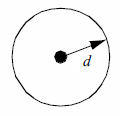
\includegraphics[width=0.96\linewidth]{Figure6-26a}
		%\caption{}
		\label{fig:Figure6-26a}
	\end{subfigure}
	\hfill
	\begin{subfigure}[h]{0.24\linewidth}
		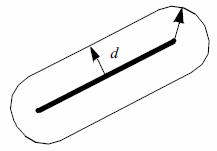
\includegraphics[width=0.96\linewidth]{Figure6-26b}
		%\caption{}
		\label{fig:Figure6-26b}
	\end{subfigure}
	\hfill
	\begin{subfigure}[h]{0.24\linewidth}
		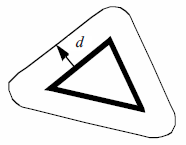
\includegraphics[width=0.96\linewidth]{Figure6-26c}
		%\caption{}
		\label{fig:Figure6-26c}
	\end{subfigure}
	\caption{Distance functions to a point, line and triangle.}\label{fig:Figure6-26}
\end{figure}

In the previous section we saw how implicit functions, or boolean combinations of implicit functions, could be used to model geometric objects. The basic approach is to evaluate these functions on a regular array of points, or volume, and then to generate scalar values at each point in the volume. Then either volume rendering (see ``Volume Rendering'' on page \pageref{sec:volume_rendering} ), or isosurface generation in combination with surface rendering, is used to display the model.

\begin{figure}[htb]
	\begin{subfigure}[h]{0.24\linewidth}
		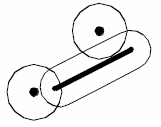
\includegraphics[width=0.96\linewidth]{Figure6-27a}
		\caption{Original}
		\label{fig:Figure6-27a}
	\end{subfigure}
	\hfill
	\begin{subfigure}[h]{0.24\linewidth}
		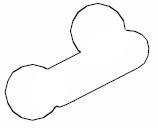
\includegraphics[width=0.96\linewidth]{Figure6-27b}
		\caption{Union}
		\label{fig:Figure6-27b}
	\end{subfigure}
	\hfill
	\begin{subfigure}[h]{0.24\linewidth}
		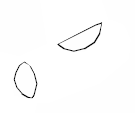
\includegraphics[width=0.96\linewidth]{Figure6-27c}
		\caption{Intersection}
		\label{fig:Figure6-27c}
	\end{subfigure}
	\begin{subfigure}[h]{0.24\linewidth}
		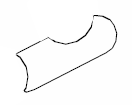
\includegraphics[width=0.96\linewidth]{Figure6-27d}
		\caption{Difference}
		\label{fig:Figure6-27d}
	\end{subfigure}
	\caption{Distance functions to a point, line and triangle.}\label{fig:Figure6-27}
\end{figure}

An extension of this approach, called implicit modeling, is similar to modeling with implicit functions. The difference lies in the fact that scalars are generated using a distance function instead of the usual implicit function. The distance function is computed as a Euclidean distance to a set of generating primitives such as points, lines, or polygons. For example, Figure \ref{fig:Figure6-26} shows the distance functions to a point, line, and triangle. Because distance functions are wellbehaved monotonic functions, we can define a series of offset surfaces by specifying different isosurface values, where the value is the distance to the generating primitive. The isosurfaces form approximations to the true offset surfaces, but using high volume resolution we can achieve satisfactory results.

Used alone the generating primitives are limited in their ability to model complex geometry. By using boolean combinations of the primitives, however, complex geometry can be easily modeled. The boolean operations union, intersection, and difference ( Equation \ref{eq:6.13}, Equation \ref{eq:6.14}, and  Equation \ref{eq:6.15}, respectively) are illustrated in Figure \ref{fig:Figure6-27}. Figure \ref{fig:Figure6-28} shows the application of implicit modeling to "thicken" the line segments in the text symbol "HELLO". The isosurface is generated on a volume $ 110 \times 40 \times 20 $ at a distance offset of $0.25$ units. The generating primitives were combined using the boolean union operator. Although Euclidean distance is always a nonnegative value, it is possible to use a signed distance function for objects that have an outside and an inside. A negative distance is the negated distance of a point inside the object to the surface of the object. Using a signed distance function allows us to create offset surfaces that are contained within the actual surface.

\begin{figure}[!htb]
	\floatbox[{\capbeside\thisfloatsetup{capbesideposition={left,center},capbesidewidth=0.4\textwidth}}]{figure}[\FBwidth]
	{\caption{Implicit modelling used to thicken a stroked font. Original lines can be seen within the translucent implicit surface.(\href{https://lorensen.github.io/VTKExamples/site/Cxx/VisualizationAlgorithms/Hello/}{Hello.cxx} or \href{https://lorensen.github.io/VTKExamples/site/Python/VisualizationAlgorithms/Hello/}{Hello.py})}\label{fig:Figure6-28}}
	{
\includegraphics[width=0.6\textwidth]{Figure6-28}}
\end{figure}

Another interesting feature of implicit modeling is that when isosurfaces are generated, more than one connected surface can result. These situations occur when the generating primitives form concave features. Figure \ref{fig:Figure6-29} illustrates this situation. If desired, multiple surfaces can be separated by using the connectivity algorithm described in ``Connectivity'' on page \pageref{subsec:connectivity}.

\begin{figure}[!htb]
	\floatbox[{\capbeside\thisfloatsetup{capbesideposition={right,center},capbesidewidth=0.4\textwidth}}]{figure}[\FBwidth]
	{\caption{Concave features can result in multiple contour lines/surfaces.}\label{fig:Figure6-29}}
	{\includegraphics[width=0.6\textwidth]{Figure6-29}}
\end{figure}
\index{implicit modelling|)}

\subsection{Glyphs}
\label{subsec:glyphs}
\index{glyph|(}

Glyphs, sometimes referred to as icons, are a versatile technique to visualize data of every type. A glyph is an ``object'' that is affected by its input data. This object may be geometry, a dataset, or a graphical image. The glyph may orient, scale, translate, deform, or somehow alter the appearance of the object in response to data. We have already seen a simple form of glyph: hedgehogs are lines that are oriented, translated and scaled according to the position and vector value of a point. A variation of this is to use oriented cones or arrows. (See ``Hedgehogs and Oriented Glyphs'' on page \pageref{subsec:hedgehogs_oriented_glyphs} for more information.)

More elaborate glyphs are possible. In one creative visualization technique Chernoff\index{Chernoff faces} \cite{Chernoff73} tied data values to an iconic representation of the human face. Eyebrows, nose, mouth, and other features were modified according to financial data values. This interesting technique built on the human capability to recognize facial expression. By tying appropriate data values to facial characteristics, rapid identification of important data points is possible.

\begin{figure}[!htb]
	\floatbox[{\capbeside\thisfloatsetup{capbesideposition={right,center},capbesidewidth=0.4\textwidth}}]{figure}[\FBwidth]
	{\caption{Glyphs indicate surface normals on model of human face. Glyph positions are randomly selected. (\href{https://lorensen.github.io/VTKExamples/site/Cxx/VisualizationAlgorithms/SpikeFran/}{SpikeFran.cxx} or \href{https://lorensen.github.io/VTKExamples/site/Python/VisualizationAlgorithms/SpikeFran/}{SpikeFran.py})}\label{fig:Figure6-30}}
	{\includegraphics[width=0.6\textwidth]{Figure6-30}}
\end{figure}

In a sense, glyphs represent the fundamental result of the visualization process. Moreover, all the visualization techniques we present can be treated as concrete representations of an abstract glyph class. For example, while hedgehogs are an obvious manifestation of a vector glyph, isosurfaces can be considered a topologically twodimensional glyph for scalar data. Delmarcelle and Hesselink \cite{Delmarcelle95} have developed a unified framework for flow visualization based on types of glyphs. They classify glyphs according to one of three categories.

\begin{itemize}

\item \emph{Elementary icons}* represent their data across the extent of their spatial domain. For example, an oriented arrow can be used to represent surface normal.

\item \emph{Local icons} represent elementary information plus a local distribution of the values around the spatial domain. A surface normal vector colored by local curvature is one example of a local icon, since local data beyond the elementary information is encoded.

\item \emph{Global icons} show the structure of the complete dataset. An isosurface is an example of a global icon.

\end{itemize}

This classification scheme can be extended to other visualization techniques such as vector and tensor data, or even to nonvisual forms such as sound or tactile feedback. We have found this classification scheme to be helpful when designing visualizations or creating visualization techniques. Often it gives insight into ways of representing data that can be overlooked.

Figure \ref{fig:Figure6-30} is an example of glyphing. Small 3D cones are oriented on a surface to indicate the direction of the surface normal. A similar approach could be used to show other surface properties such as curvature or anatomical keypoints.
\index{glyph|)}

\subsection{Cutting}
\label{subsec:cutting}
\index{cutting!with implicit functions|(}

Often we want to cut through a dataset with a surface and then display the interpolated data values on the surface. We refer to this technique as \emph{data cutting} or simply \emph{cutting}. The data cutting operation requires two pieces of information: a definition for the surface and a dataset to cut. We will assume that the cutting surface is defined by an implicit function. A typical application of cutting is to slice through a dataset with a plane, and color map the scalar data and/or warp the plane according to vector value.

\begin{figure}[!htb]
	\floatbox[{\capbeside\thisfloatsetup{capbesideposition={left,center},capbesidewidth=0.4\textwidth}}]{figure}[\FBwidth]
	{\caption{ Cut through structured grid with plane. The cut plane is shown solid shaded. A computational plane of constant value is shown in wireframe for comparison. The colors correspond to flow density. Cutting surfaces are not necessarily planes: implicit functions such as spheres, cylinders, and quadrics can also be used. (\href{https://lorensen.github.io/VTKExamples/site/Cxx/VisualizationAlgorithms/CutStructuredGrid/}{CutStructuredGrid.cxx} or \href{https://lorensen.github.io/VTKExamples/site/Python/VisualizationAlgorithms/CutStructuredGrid/}{CutStructuredGrid.py})}\label{fig:Figure6-31}}
	{\includegraphics[width=0.6\textwidth]{Figure6-31}}
\end{figure}

A property of implicit functions is to convert a position into a scalar value (see ``Implicit Functions`` on page \pageref{subsec:implicit_functions} ). We can use this property in combination with a contouring algorithm (e.g., marching cubes\index{marching cubes!and cut surfaces}) to generate cut surfaces. The basic idea is to generate scalars for each point of each cell of a dataset (using the implicit cut function), and then contour the surface value $F(x,y,z) = 0$.

The cutting algorithm proceeds as follows. For each cell, function values are generated by evaluating $F(x,y,z)$ for each cell point. If all the points evaluate positive or negative, then the surface does not cut the cell. However, if the points evaluate positive and negative, then the surface passes through the cell. We can use the cell contouring operation to generate the isosurface $F(x,y,z) = 0$. Data attribute values can then be computed by interpolating along cut edges.

\begin{figure}[htb]
	\begin{subfigure}[h]{0.48\linewidth}
		%\includegraphics[width=0.96\linewidth]{Figure6-32a}
		\caption{}
		\label{fig:Figure6-32a}
	\end{subfigure}
	\hfill
	\begin{subfigure}[h]{0.48\linewidth}
		\includegraphics[width=0.96\linewidth]{Figure6-32b}
		\caption{}
		\label{fig:Figure6-32b}
	\end{subfigure}
	\caption{100 cut planes with opacity of 0.05. Rendered back--to--front to simulate	volume rendering.(\href{https://lorensen.github.io/VTKExamples/site/Cxx/VolumeRendering/PseudoVolumeRendering}{PseudoVolumeRendering.cxx} or \href{https://lorensen.github.io/VTKExamples/site/Python/VolumeRendering/PseudoVolumeRendering/}{PseudoVolumeRendering.py})}\label{fig:Figure6-32}
\end{figure}

Figure \ref{fig:Figure6-31} illustrates a plane cut through a structured grid dataset. The plane passes through the center of the dataset with normal $(-0.287, 0, 0.9579)$. For comparison purposes a portion of the grid geometry is also shown. The grid geometry is the grid surface $k=9$ (shown in wireframe). A benefit of cut surfaces is that we can view data on (nearly) arbitrary surfaces. Thus, the structure of the dataset does not constrain how we view the data.

We can easily make multiple planar cuts through a structured grid dataset by specifying multiple isovalues for the cutting algorithm. Figure \ref{fig:Figure6-32} shows $100$ cut planes generated perpendicular to the camera's view plane normal. Rendering the planes from back to front with an opacity of $0.05$ produces a simulation of volume rendering (see ``Volume Rendering'' on page \pageref{sec:volume_rendering} ).

\begin{figure}[!htb]
	\floatbox[{\capbeside\thisfloatsetup{capbesideposition={right,center},capbesidewidth=0.4\textwidth}}]{figure}[\FBwidth]
	{\caption{Cutting a surface model of the skin with a series of planes produces contour lines. Lines are wrapped with tubes for clarity. (\href{https://lorensen.github.io/VTKExamples/site/Cxx/VisualizationAlgorithms/CutWithScalars/}{CutWithScalars.cxx} or \href{https://lorensen.github.io/VTKExamples/site/Python/VisualizationAlgorithms/CutWithScalars/}{CutWithScalars.py})}\label{fig:Figure6-33}}
	{\includegraphics[width=0.6\textwidth]{Figure6-33}}
\end{figure}

This example illustrates that cutting the volumetric data in a structured grid dataset produced polygonal cells. Similarly, cutting polygonal data produces lines. Using a single plane equation, we can extract ``contour lines'' from a surface model defined with polygons. Figure \ref{fig:Figure6-33} shows contours extracted from a surface model of the skin. At each vertex in the surface model we evaluate the equation of the plane and $F(x.y.z) = c$ and store the valuec of the function as a scalar value. Cutting the data with $46$ isovalues from $1.5$ to $136.5$ produces contour lines that are $3$ units apart.
\index{cutting!with implicit functions|)}
\index{algorithms!modelling|)}

\section{Putting It All Together}

Algorithms are implemented in the \emph{Visualization Toolkit} as process objects. These objects may be either sources, filters, or mappers (see ``The Visualization Pipeline'' on page \pageref{sec:visualization_pipeline} ). In this section we will describe how these objects are implemented.

\subsection{Process Object Design}

\begin{description}[leftmargin=0cm,labelindent=0cm]

\item[Source Design.]
Source objects have no visualization data for input and one or more outputs, Figure \ref{fig:Figure6-34} illustrates this for the concrete source object vtkSphereSource. This class inherits from vtkPolyDataAlgorithm, indicating that it creates polygonal data on output.

The convenience object vtkPolyDataAlgorithm has been created to simplify subclass derivation. For example, vtkBYUReader is also a type of vtkPolyDataAlgorithm. The major difference between vtkSphereSource and vtkBYUReader is the implementation of the virtual method RequestData(). This method actually creates its output data. If you derive a source object you do not need to make it a subclass of any convenience object (e.g., vtkPolyDataAlgorithm), but you should derive it from vtkAlgorithm.

\begin{figure}[htb]
	\begin{subfigure}[h]{0.48\linewidth}
		\includegraphics[width=0.96\linewidth]{Figure6-34a}
		\caption{Functional model}
		\label{fig:Figure6-34a}
	\end{subfigure}
	\hfill
	\begin{subfigure}[h]{0.48\linewidth}
		\includegraphics[width=0.96\linewidth]{Figure6-34b}
		\caption{Object model}
		\label{fig:Figure6-34b}
	\end{subfigure}
	\caption{Source object design. Example shown is a source object that creates a polygonal representation of a sphere.}\label{fig:Figure6-34}
\end{figure}

\item[Filter Design.]
\index{filter object!implementation|(}

Filter objects have one or more inputs and one or more outputs as shown in Figure \ref{fig:Figure6-34}. (You may also refer to ``Pipeline Design and Implementation'' on page \pageref{subsec:pipeline_design_implementation}.) To create Figure \ref{fig:Figure6-35} a filter object, inheritance is used to specify the type of input and output data objects. illustrates this for the concrete source object vtkContourFilter (which implements marching cubes\index{marching cubes!implementation} and other contouring techniques). It is worth examining this object diagram in detail since it is the basis for the architecture of the visualization pipeline.

The superclasses of vtkContourFilter are vtkAlgorithm and vtkPolyDataAlgorithm. The class vtkPolyDataAlgorithm specifies the type of data vtkContourFilter produces on output (i.e., a vtkPolyData ). Because this filter should take any subclass of vtkDataSet as input, it must override its superclasses implementation of the FillInputPortInformation() method to specify this. Note that inheritance from vtkPolyDataAlgorithm is optional --- this functionality could be implemented directly in vtkContourFilter. This optional superclass is simply a convenience object to make class derivation a little easier.

What is left for vtkContourFilter to implement is its RequestData() method (as well as constructor, print method, and any other methods special to this class). Thus the primary difference between classes with equivalent inheritance hierarchies is the implementation of the RequestData() method.

Subclasses of vtkAlgorithm enforce filter input and output type by use of the FillInputPortInformation() and FillOutputPortInformation() methods. By default, its subclass vtkDataSetAlgorithm accepts input type vtkDataSet (or subclasses) and produces a vtkDataSet on output. (The type of the output is determined by the type of the input.) Since vtkDataSet is a base class for all data types, subclasses of vtkDataSetAlgorithm will accept any type as input. Specialized filters are derived from other classes. For example, filters that accept polygonal data might be derived from vtkPolyDataAlgorithm, and filters that accept unstructured grid datasets might be derived from vtkUnstructuredGridAlgorithm.

We encourage you to examine the source code carefully for a few filter and source objects.

The architecture is simple enough that you can grasp it quickly.

\begin{figure}[htb]
	\begin{subfigure}[h]{0.48\linewidth}
		\includegraphics[width=0.96\linewidth]{Figure6-35a}
		\caption{Functional model}
		\label{fig:Figure6-35a}
	\end{subfigure}
	\hfill
	\begin{subfigure}[h]{0.48\linewidth}
		\includegraphics[width=0.96\linewidth]{Figure6-35b}
		\caption{Object model}
		\label{fig:Figure6-35b}
	\end{subfigure}
	\caption{Filter object design. The example shown is for an object that receives a general dataset as input and creates polygonal data on output.}\label{fig:Figure6-35}
\end{figure}

\begin{figure}[htb]
	\begin{subfigure}[h]{0.48\linewidth}
		\begin{subfigure}[h]{0.48\linewidth}
			\includegraphics[width=0.96\linewidth]{Figure6-36a}
			\label{fig:Figure6-36a}
		\end{subfigure}
		\hfill
		\begin{subfigure}[h]{0.48\linewidth}
			\includegraphics[width=0.96\linewidth]{Figure6-36b}
			\label{fig:Figure6-36b}
		\end{subfigure}
		\caption{Functional models}
	\end{subfigure}
	\hfill
	\begin{subfigure}[h]{0.48\linewidth}
		\begin{subfigure}[h]{0.48\linewidth}
			\includegraphics[width=0.96\linewidth]{Figure6-36c}
			\label{fig:Figure6-36c}
		\end{subfigure}
		\begin{subfigure}[h]{0.48\linewidth}
			\includegraphics[width=0.96\linewidth]{Figure6-36d}
			\label{fig:Figure6-36d}
		\end{subfigure}
		\caption{Object models}
	\end{subfigure}
	\caption{Mapper object design. Graphics mapper shown (e.g., vtkPolyDataMapper) maps polygonal data through graphics library primitives. Writer shown (e.g., vtkSTLWriter) writes polygonal data to stereo lithography format.}\label{fig:Figure6-36}
\end{figure}
\index{filter object!implementation|)}

\item[Mapper Design.]
\label{subsubsec:mapper_design}
\index{mapper object!implementation|(}

Mapper objects have one or more inputs and no visualization data output, Figure \ref{fig:Figure6-36}. Two different types of mappers are available in the \emph{Visualization Toolkit}: graphics mappers and writers. Graphics mappers interface geometric structure and data attributes to the graphics library; writers write datasets to disk or other I/O devices.

Since mappers take datasets as input, type enforcement is required. Each mapper implements this functionality directly. For example, both classes vtkPolyDataMapper and vtkSTLWriter implement a SetInput() method to enforce the input to be of type vtkPolyData. Other mappers and writers enforce input type as appropriate.

Although writers and mappers do not create visualization data, they both have methods similar to the RequestData() method of the sources and filters. Each subclass of vtkMapper must implement the Render() method. This method is exchanged by the graphics system actors and its associated mappers during the rendering process. The effect of the method is to map its input dataset to the appropriate rendering library/system. Subclasses of the class vtkWriter must implement the WriteData() method. This method causes the writer to write its input dataset to disk (or other I/O device).
\index{mapper object!implementation|)}

\end{description}

\subsubsection{Color Maps}
\index{color mapping!implementation|(}

Color maps are created in the Visualization Toolkit using instances of the class vtkLookupTable. This class allows you to create a lookup table using HSVA (e.g., hue, saturation, value, and alpha opacity) specification. Although we discussed the HSV color system in Chapter 3: \nameref{chap:computer_graphics_primer}, we haven't yet defined alpha opacity. We shall do so in Chapter 7:  \nameref{chap:advanced_computer_graphics}, but until then consider the alpha value to be the opacity of an object. Alpha values of one indicate that the object is opaque, while alpha values of zero indicate that the object is transparent.

The procedure for generating lookup table entries\index{lookup table!implementation} is to define pairs of values for HSVA. These pairs define a linear ramp for hue, saturation, value, and opacity. When the Build() method is invoked, these linear ramps are used to generate a table with the number of table entries requested. Alternatively, vtkLookupTable also enables you to load colors directly into the table. Thus, you build custom tables that cannot be simply expressed as linear ramps of HSVA values. To demonstrate this procedure, we specify a starting and ending value for each of the components of HSVA, then we will create a rainbow lookup table from blue to red by using the following C++ code.

\begin{lstlisting}[language=C++, caption={Create a rainbow lookup table.}]
vtkLookupTable *lut = vtkLookupTable::New();
  lut->SetHueRange(0.6667, 0.0);
  lut->SetSaturationRange(1.0, 1.0);
  lut->SetValueRange(1.0, 1.0);
  lut->SetAlphaRange(1.0, 1.0);
  lut->SetNumberOfColors(256);
  lut->Build();
\end{lstlisting}

Since the default values for SaturationRange, ValueRange, AlphaRange, and the number of lookup table colors are $(1,1)$, $(1,1)$, $(1,1)$, and $256$, respectively, we can simplify this process to the following

\begin{lstlisting}[language=C++, caption={Create a rainbow lookup table (simplified).}]
vtkLookupTable *lut = vtkLookupTable::New();
  lut->SetHueRange(0.6667, 0.0);
  lut->Build();
\end{lstlisting}

(The default values for HueRange are $(0.0, 0.6667)$ --- a red to blue color table.)

To build a black and white lookup table of 256 entries we use

\begin{lstlisting}[language=C++, caption={Create a black and white lookup table.}]
vtkLookupTable *lut = vtkLookupTable::New();
  lut->SetHueRange(0.0, 0.0);
  lut->SetSaturationRange(0.0, 0.0);
  lut->SetValueRange(0.0, 1.0)
\end{lstlisting}

In some cases you may want to specify colors directly. You can do this by specifying the number of colors, building the table, and then inserting new colors. When you insert colors, the RGBA color description system is used. For example, to create a lookup table of the three colors red, green, and blue, use the following C++ code.

\begin{lstlisting}[language=C++, caption={Directly specifying colors.}]
vtkLookupTable *lut = vtkLookupTable::New();
  lut->SetNumberOfColors(3);
  lut->Build();
  lut->SetTableValue(0, 1.0, 0.0, 0.0, 1.0);
  lut->SetTableValue(0, 0.0, 1.0, 0.0, 1.0);
  lut->SetTableValue(0, 0.0, 0.0, 1.0, 1.0);
\end{lstlisting}

Lookup tables in the \emph{Visualization Toolkit} are associated with the graphics mappers. Mappers will automatically create a red to blue lookup table if no table is specified, but if you want to create your own, use the \sloppy{\lstinline{mapper->SetLookupTable(lut)}} operation where mapper is an instance of vtkMapper or its subclasses.

A few final notes on using lookup tables.

\begin{itemize}

\item  Mappers use their lookup table to map scalar values to colors. If no scalars are present, the mappers and their lookup tables do not control the color of the object. Instead the vtkProperty object associated with the vtkActor class does. Use vtkProperty's method \sloppy{\lstinline{actor->GetProperty()->SetColor(r,g,b)}} where r, g, and b are floating point values specifying color.

\item If you want to prevent scalars from coloring your object, use vtkMapper's method \sloppy{\lstinline{mapper->ScalarVisibilityOff()}} to turn off color mapping. Then the actor's color will control the color of the object.

\item The scalar range (i.e., the range into which the colors are mapped) is specified with the mapper. Use the method \sloppy{\lstinline{mapper->SetScalarRange(min, max)}}.

\end{itemize}

You can also derive your own lookup table types. Look at vtkLogLookupTable for an example. This particular lookup table inherits from vtkLookupTable. It performs logarithmic mapping of scalar value to table entry, a useful capability when scalar values span many orders of magnitude.
\index{color mapping!implementation|)}

\subsubsection{Implicit Functions}
\index{implicit function!implementation|(}

As we have seen, implicit functions can be used for visualizing functions, creating geometry, and cutting or selecting datasets. VTK includes several implicit functions including a single plane (vtkPlane ), multiple convex planes ( vtkPlanes ), spheres ( vtkSphere ), cones ( vtkCone ), cylinders (vtkCylinder ), and the general quadric ( vtkQuadric ). The class vtkImplicitBoolean allows you to create boolean combinations of these implicit function primitives. Other implicit functions can be added to VTK by deriving from the abstract base class vtkImplicitFunction.

\begin{figure}[htb]
	\includegraphics[width=0.96\linewidth]{Figure6-37}
	\caption{Inheritance hierarchy of vtkImplicitFunction and subclasses.}\label{fig:Figure6-37}
\end{figure}

The existing inheritance hierarchy for implicit functions is shown in Figure \ref{fig:Figure6-37}. Subclasses of vtkImplicitFunction must implement the two methods Evaluate() and Gradient(x). The method Evaluate() returns the value of the function at point $(x,y,z)$, while the method Gradient() returns the gradient vector to the function at point $(x,y,z)$.
\index{implicit function!implementation|)}

\subsubsection{Contouring}
\index{contouring!implementation|(}\index{isosurface!implementation|(}\index{marching cubes!implementation|(}

Scalar contouring is implemented in the Visualization Toolkit with vtkContourFilter. This filter object accepts as input any dataset type. Thus, vtkContourFilter treats every cell type and each cell type must provide a method for contouring itself.

Contouring in VTK is implemented using variations of the marching cubes algorithm presented earlier. That is, a contour case table is associated with each cell type, so each cell will generate contouring primitives as appropriate. For example, the tetrahedron cell type implements ``marching tetrahedron'' and creates triangle primitives, while the triangle cell type implements ``marching triangles'' and generates lines segments.

The implication of this arrangement is that vtkContourFilter will generate point, line, and surface contouring primitives depending on the combination of input cell types. Thus vtkContourFilter is completely general. We have created another contour filter, vtkMarchingCubes, that is specific to the dataset type image data (in particular, 3D volumes). These two filters allow us to compare (at least for this one algorithm) the cost of generality.

Recall from ``Generality Versus Efficiency'' on page \pageref{subsec:benerality_vs_efficiency} the issues regarding the trade--offs between general and specific algorithms. Figure \ref{fig:Figure6-38} shows a comparison of CPU times for a volume dataset at $64 \times 64\times 93$, $128 \times 128\times 93$ and $256 \times 256\times 93$. The volume is a CT dataset of a human head. Three cases were run. In the first case the  vtkMarchingCubes object was used\index{marching cubes!general versus specific}. The output of this filter is triangles plus point normals. In the second case, vtkContourFilter was run. The output of this filter is just triangles. In the last case, vtkContourFilter was combined with vtkPolyDataNormals (to generate point normals). The output of the combined filters is also triangles plus point normals.

The execution times are normalized to the smallest dataset using the vtkMarchingCubes object. The results are clear: The specific object outperforms the general object by a factor of $1.4$ to $7$, depending on data size and whether normals are computed. The larger differences occur on the smaller datasets. This is because the ratio of voxel cells containing the isosurface to the total number of voxels is larger for smaller datasets. (Generally the total number of voxels increases as the resolution cubed, while the voxels containing the isosurface increase as the resolution squared.) As a result, more voxels are processed in the smaller datasets relative to the total number of voxels than in the larger datasets. When the datasets become larger, more voxels are ``empty'' and are not processed.

Although these results do not represent all implementations or the behavior of other algorithms, they do point to the cost of generality. Of course, there is a cost to specialization as well. This cost is typically in programmer time, since the programmer must rewrite code to adapt to new circumstances and data. Like all trade--offs, resolution of this issue requires knowledge of the application.

\begin{figure}[!htb]
	\begin{subfigure}[h]{0.32\linewidth}
		\includegraphics[width=0.96\linewidth]{Figure6-38a}
		\caption{Quarter resolution}
		\label{fig:Figure6-38a}
	\end{subfigure}
	\hfill
	\begin{subfigure}[h]{0.32\linewidth}
		\includegraphics[width=0.96\linewidth]{Figure6-38b}
		\caption{Half resolution}
		\label{fig:Figure6-38b}
	\end{subfigure}
	\hfill
	\begin{subfigure}[h]{0.32\linewidth}
		\includegraphics[width=0.96\linewidth]{Figure6-38c}
		\caption{Full resolution}
		\label{fig:Figure6-38c}
	\end{subfigure}
	\hfill
	\begin{subfigure}[h]{0.96\linewidth}
		\caption*{}
	\end{subfigure}
	\hfill
	\begin{subfigure}[h]{0.96\linewidth}
		\begin{tabular}{|c|d{2.3}|d{2.3}|d{2.3}|d{2.3}|d{2.3}|}
			\hline
			Resolution & \multicolumn{1}{c|}{Specific} & \multicolumn{1}{c|}{General} & \multicolumn{1}{c|}{Factor} & \multicolumn{1}{c|}{General} & \multicolumn{1}{c|}{Factor} \\
			& \multicolumn{1}{c|}{(w/ normals)} & \multicolumn{1}{c|}{(no normals)} & \multicolumn{1}{c|}{Factor} & \multicolumn{1}{c|}{(w normals)} &  \\
			\hline
			$64 \times 64\times 93$ & 1.000 & 2.889 & 2.889 & 7.131 & 7.131 \\
			$128 \times 128 \times 93$ & 5.058 & 11.810 & 2.330 & 23.360 & 4.600 \\
			$256 \times 256\times 93$ & 37.169 & 51.160 & 1.390 & 87.230 & 2.350 \\
			\hline
		\end{tabular}
		\caption*{}
		\label{fig:Figure6-38d}
	\end{subfigure}
	\caption{The cost of generality. Isosurface generation of three volumes of different sizes are
		compared. The results show normalized execution times for two different implementations of the
		marching-cubes isosurface algorithm. The specialized filter is \emph{vtkMarchingCubes}. The general
		algorithms are first \emph{vtkContourFilter} and then in combination with \emph{vtkPolyDataNormals}.}\label{fig:Figure6-38}
\end{figure}

\begin{figure}[!htb]
	\begin{subfigure}[h]{0.48\linewidth}
		\includegraphics[width=0.96\linewidth]{Figure6-39a}
		\caption*{}
		\label{fig:Figure6-39a}
	\end{subfigure}
	\hfill
	\begin{subfigure}[h]{0.48\linewidth}
		\includegraphics[width=0.96\linewidth]{Figure6-39b}
		\caption*{(\href{https://lorensen.github.io/VTKExamples/site/Cxx/VisualizationAlgorithms/ContourQuadric/}{ContourQuadric.cxx} or \href{https://lorensen.github.io/VTKExamples/site/Python/VisualizationAlgorithms/ContourQuadric/}{ContourQuadric.py})}
		\label{fig:Figure6-39b}
	\end{subfigure}
	\hfill
	\begin{subfigure}[h]{0.96\linewidth}
		\caption*{}
	\end{subfigure}
	\hfill
	\begin{subfigure}[h]{0.96\linewidth}
		\begin{lstlisting}[language=C++, caption={}]
		// Define implicit function
		vtkQuadric *quadric = vtkQuadric::New();
		  quadric->SetCoefficients(.5,1,.2,0,.1,0,0,.2,0,0);
		vtkSampleFunction *sample = vtkSampleFunction::New();
		  sample->SetSampleDimensions(50,50,50);
		  sample->SetImplicitFunction(quadric);
		vtkContourFilter *contour = vtkContourFilter::New();
		  contour->SetInputConnection(sample->GetOutputPort());
		  contour->GenerateValues(5,0,1.2);
		vtkPolyDataMapper *contourMapper = vtkPolyDataMapper::New();
		  contourMapper->SetInputConnection( contour->GetOutputPort());
		  contourMapper->SetScalarRange(0,1.2);
		vtkActor *contourActor = vtkActor::New();
		  contourActor->SetMapper(contourMapper);
		// Create outline
		vtkOutlineFilter *outline = vtkOutlineFilter::New();
		  outline->SetInputConnection(sample->GetOutputPort());
		vtkPolyDataMapper *outlineMapper = vtkPolyDataMapper::New();
		  outlineMapper->SetInputConnection(outline->GetOutputPort());
		vtkActor *outlineActor = vtkActor::New();
		  outlineActor->SetMapper(outlineMapper);
		  outlineActor->GetProperty()->SetColor(0,0,0);
		\end{lstlisting}
		\caption*{}
		\label{fig:Figure6-39c}
	\end{subfigure}
	\caption{Contouring quadric function. Pipeline topology, C++ code, and resulting image are shown.}\label{fig:Figure6-39}
\end{figure}

An example use of vtkContourFilter is shown in Figure \ref{fig:Figure6-39}. This example is taken from Figure \ref{fig:Figure4-1}, which is a visualization of a quadric function. The class vtkSampleFunction samples the implicit quadric function using the vtkQuadric class. Although vtkQuadric does not participate in the pipeline in terms of data flow, it is used to define and evaluate the quadric function. It is possible to generate one or more isolines/isosurfaces simultaneously using vtkContourFilter. As Figure \ref{fig:Figure6-39} shows, we use the GenerateValues() method to specify a scalar range, and the number of contours within this range (including the initial and final scalar values). vtkContourFilter generates duplicate vertices, so we can use vtkCleanPolyData to remove them. To improve the rendered appearance of the isosurface, we use vtkPolyDataNormals to create surface normals. (We describe normal generation in Chapter 9: \nameref{chap:advanced_algorithms}.)

\begin{figure}[!htb]
	\floatbox[{\capbeside\thisfloatsetup{capbesideposition={right,center},capbesidewidth=0.4\textwidth}}]{figure}[\FBwidth]
	{\caption{Data flow into and out of the \emph{vtkGlyph3D} class.}\label{fig:Figure6-40}}
	{\includegraphics[width=0.6\textwidth]{Figure6-40}}
\end{figure}
\index{contouring!implementation|)}\index{isosurface!implementation|)}\index{marching cubes!implementation|)}


\subsection{Cutting}
\index{cutting!implementation|(}

The vtkCutter class performs cutting of all VTK cell types. The SetValue() and GenerateValues() methods permit the user to specify which multiple scalar values to use for the cutting. vtkCutter requires an implicit function that will be evaluated at each point in the dataset. Then each cell is cut using the cell's Contour method. Any point attributes are interpolated to the resulting cut vertices. The sorting order for the generated polygonal data can be controlled with the SortBy method. The default sorting order, SortByValue(), processes cells in the inner loop for each contour value. SortByCell() processes the cutting value in the inner loop and produces polygonal data that is suitable for backtofront rendering (see Figure \ref{fig:Figure6-32}). (The sorting order is useful when rendering with opacity as discussed in Chapter 7:  \nameref{chap:advanced_computer_graphics}.) Notice the similarity of this filter to the vtkContourFilter. Both of these objects contour datasets with multiple isovalues. vtkCutter uses an implicit function to calculate scalar values while vtkContourFilter uses the scalar data associated with the dataset's point data.
\index{cutting!implementation|)}

\subsection{Glyphs}
\index{glyph!implementation|(}

The vtkGlyph3D class provides a simple, yet powerful glyph capability in the \emph{Visualization Toolkit}. vtkGlyph3D is an example of an object that takes multiple inputs (Figure \ref{fig:Figure6-40}). One input, specified with the SetInputConnection() method, defines a set of points and possible attribute data at those points. The second input, specified with the SetSourceConnection() method, defines a geometry to be copied to every point in the input dataset. The source is of type vtkPolyData. Hence, any filter, sequence of filters creating polygonal data, or a polygonal dataset may be used to describe the glyph's geometry.

The behavior of an instance of vtkGlyph3D depends on the nature of the input data and the value of its instance variables. Generally, the input Source geometry will be copied to each point of the Input dataset. The geometry will be aligned along the input vector data and scaled according to the magnitude of the vector or the scalar value. In some cases, the point normal is used rather than the vector. Also, scaling can be turned on or off.

We saw how to use vtkGlyph3D in the example given in Figure \ref{fig:Figure4-20}. Cones were used as the glyph and were located at each point on the sphere, oriented along the sphere's surface normal.
\index{glyph!implementation|)}

\subsection{Streamlines}

\begin{figure}[!htb]
	\floatbox[{\capbeside\thisfloatsetup{capbesideposition={left,center},capbesidewidth=0.4\textwidth}}]{figure}[\FBwidth]
	{\caption{Inheritance hierarchy for vtkStreamer and subclasses.}\label{fig:Figure6-41}}
	{\includegraphics[width=0.6\textwidth]{Figure6-41}}
\end{figure}

Streamlines and particle motion require numerical integration to guide a point through the vector field. Vector visualization algorithms that we will see in later chapters also require numerical integration. As a result, we designed an object hierarchy that isolates the numerical integration process into a single base class. The base class is vtkStreamer and it is responsible for generating a particle path through a vector field of specified length (expressed as elapsed time). Each derived class of vtkStreamer takes advantage of this capability to move through the vector field but implements its own particular representational technique to depict particle motion. Streamlines ( vtkStreamLine ) draw connected lines while particle motion is shown by combining the output of vtkStreamPoints with the vtkGlyph3D object. Using vtkGlyph3D we can place spheres or oriented objects such as cones or arrows at points on the particle path created by vtkStreamPoints. The inheritance hierarchy for vtkStreamer and subclasses is shown in  Figure \ref{fig:Figure4-20}.

The integration method in vtkStreamer is implemented as a virtual function. Thus it can be overloaded as necessary. Possible reasons for overloading include implementing an integration technique of higher or lower accuracy, or creating a technique specialized to a particular dataset type. For example, the search process in a volume is much faster than it is for other dataset types, therefore, highly efficient vector integration techniques can be constructed.

The vector integration technique in VTK will accommodate any cell type. Thus, integration through cells of any topological dimension is possible. If the cells are of topological dimension 2 or less, the integration process constrains particle motion to the surface (2D) or line (1D). The particle may only leave a cell by passing through the cell boundary, and traveling to a neighboring cell, or exiting the dataset.

\subsection{Abstract Filters}

Attribute transformations create or modify data attributes without changing the topology or geometry of a dataset. Hence filters that implement attribute transformation (e.g., vtkElevationFilter ) can accept any dataset type as input, and may generate any dataset type on output. Unfortunately, because filters must specialize the particular type of data they output, at first glance it appears that filters that create general dataset types on output are not feasible. This is because the type vtkDataSet is an abstract type and must be specialized to allow instantiation.

\begin{figure}[!htb]
	\includegraphics[width=0.96\linewidth]{Figure6-42}
	\caption{Depiction of data flow for abstract filter output. The output object type is the same as the input type.}\label{fig:Figure6-42}
\end{figure}


Fortunately, there is a solution to this dilemma. The solution is to use the ``virtual constructor'' NewInstance(). Although C++ does not allow virtual constructors, we can simulate it by creating a special virtual function that constructs a copy of the object that it is invoked on. For example, if this function is applied to a dataset instance of type vtkPolyData, the result will be a copy of that instance (Figure \ref{fig:Figure6-42} ). (Note that we use reference counting to make copies and avoid duplicating memory.) The virtual constructor function NewInstance() is implemented in a number of VTK classes including datasets and cells.

Using the virtual constructor we can construct filters that output abstract data types like vtkDataSet. We simply apply NewInstance() to the input of the filter. This will then return a pointer to a concrete object that is the output of the filter. The result is a general filter object that can accept any dataset type for input and creates the general vtkDataSet type as output. In VTK, this functionality has been implemented in the abstract class vtkDataSetAlgorithm.

There are other filters that implement variations of this delegation technique. The class vtkPointSetAlgorithm is similar to vtkDataSetAlgorithm. This class takes as input any dataset whose geometry is explicitly defined via an instance of vtkPoints (or subclass), and generates on output an object of the same type (i.e., vtkPointSet ). The class vtkMergeFilter combines dataset structure and point attributes from one or more input datasets. For example, you can read multiple files and combine the geometry/topology from one file with different scalars, vectors, and normals from other files.

One difficulty using abstract filter types is that the output type may not match with the input type of a downstream filter. For example, the output of vtkElevationFilter is specified as vtkDataSet even though the input may be of type vtkPolyData, and we know from the previous discussion that the actual output type will be vtkPolyData. This difficulty is removed by using the filter vtkCastToConcrete\index{casting!VTK data types}, which allows you to runtime cast to the appropriate output type. In this case we would use the GetPolyDataOutput() from vtkCastToConcrete. After checking the validity of the cast, this method returns a dataset cast to vtkPolyData. Of course, this process requires that the input to vtkCastToConcrete be set before the output is requested.

\subsection{Visualizing Blood Flow}

In this example we'll combine a few different techniques to visualize blood flow in the human carotid arteries. Our data contains both vectors that represent the velocity of blood and scalars that are proportional to the magnitude of the velocity (i.e., speed).

We can provide context for the visualization by creating an isosurface of speed. This isosurface shows regions of fastest blood flow, and is similar to, but not the same as, the actual surface of the arteries. However, it provides us with a visual cue to the structure of the arteries. The first vector visualization technique we'll use is to generate vector glyphs ( Unfortunately, we cannot just create glyphs at each point because of the number of points (over 167,000 points). To do so would result in a confusing mess, and the interactive speed would be poor. Instead, we'll use two filters to select a subset of the available points. These filters are vtkThresholdPoints and vtkMaskPoints.

vtkThresholdPoints allows us to extract points that satisfy a certain threshold criterion. In our example, we choose points whose speed is greater than a specified value. This eliminates a large number of points, since most points lie outside the arteries and have a small speed value.

The filter vtkMaskPoints allows us to select a subset of the available points. We specify the subset with the OnRatio instance variable. This instance variable indicates that every OnRatio point is to be selected. Thus, if the OnRatio is equal to one, all points will be selected, and if the OnRatio is equal to ten, every tenth point will be selected. This selection can be either uniform or random. Random point selection is set using the RandomModeOn() and RandomModeOff() methods.

After selecting a subset of the original points, we can use the vtkGlyph3D filter in the usual way. A cone's orientation indicates blood flow direction, and its size and color correspond to the velocity magnitude. Figure \ref{fig:Figure6-43} shows the pipeline, sample code, and a resulting image from this visualization. Note that we've implemented the example using the interpreted language Tcl. See Chapter 11: \nameref{chap:visualization_web} if you want more information about Tcl.

\begin{figure}[!htb]
	\begin{subfigure}[h]{0.48\linewidth}
		\includegraphics[width=0.96\linewidth]{Figure6-43a}
		\caption*{}
		\label{fig:Figure6-43a}
	\end{subfigure}
	\hfill
	\begin{subfigure}[h]{0.48\linewidth}
		\includegraphics[width=0.96\linewidth]{Figure6-43b}
		\caption*{(\href{https://lorensen.github.io/VTKExamples/site/Cxx/VisualizationAlgorithms/CarotidFlowGlyphs/}{CarotidFlowGlyphs.cxx} or \href{https://lorensen.github.io/VTKExamples/site/Python/VisualizationAlgorithms/CarotidFlowGlyphs/}{CarotidFlowGlyphs.py})}
		\label{fig:Figure6-43b}
	\end{subfigure}
	\hfill
	\begin{subfigure}[h]{0.96\linewidth}
		\caption*{}
	\end{subfigure}
	\hfill
	\begin{subfigure}[h]{0.96\linewidth}
		\begin{lstlisting}[language=TCL, caption={}]
		vtkStructuredPointsReader reader
		  reader SetFileName "$env(VTK_TEXTBOOK_DATA)/carotid.vtk"
		vtkThresholdPoints threshold
		  threshold SetInputConnection [reader GetOutputPort]
		  threshold ThresholdByUpper 200
		vtkMaskPoints mask
		  mask SetInputConnection [Threshold GetOutputPort]
		  mask SetOnRatio 10
		vtkConeSource cone
		  cone SetResolution 3
		  cone SetHeight 1
		  cone SetRadius 0.25
		vtkGlyph3D cones
		  cones SetInputConnection [mask GetOutputPort]
		  cones SetSourceConnection [cone GetOutputPort]
		  cones SetScaleFactor 0.5
		  cones SetScaleModeToScaleByVector
		vtkLookupTable lut
		  lut SetHueRange.667 0.0
		  lut Build
		vtkPolyDataMapper vecMapper
		  vecMapper SetInputConnection [cones GetOutputPort]
		  vecMapper SetScalarRange 2 10
		  vecMapaper SetLookupTable lut
		\end{lstlisting}
		\caption*{}
		\label{fig:Figure6-43c}
	\end{subfigure}
	\caption{Visualizing blood flow in human carotid arteries. Cone glyphs indicate flow direction and magnitude.}\label{fig:Figure6-43}
\end{figure}

In the next part of this example we'll generate streamtubes of blood velocity. Again we use an isosurface of speed to provide us with context. The starting positions for the streamtubes were determined by experimenting with the data. Because of the way the data was measured and the resolution of the velocity field, many streamers travel outside the artery. This is because the boundary layer of the blood flow is not captured due to limitations in data resolution. Consequently, as the blood flows around curves, there is a component of the velocity field that directs the streamtube outside the artery. As a result it is hard to find starting positions for the streamtubes that yield interesting results. We use the source object vtkPointSource in combination with vtkThresholdPoints to work around this problem. vtkPointSource generates random points centered around a sphere of a specified radius. We need only find an approximate position for the starting points of the streamtubes and then generate a cloud of random seed points. vtkThresholdPoints is used to cull points that may be generated outside the regions of high flow velocity.

\begin{figure}[!htb]
	\begin{subfigure}[h]{0.48\linewidth}
		\includegraphics[width=0.96\linewidth]{Figure6-44a}
		\caption*{}
		\label{fig:Figure6-44a}
	\end{subfigure}
	\hfill
	\begin{subfigure}[h]{0.48\linewidth}
		\includegraphics[width=0.96\linewidth]{Figure6-44b}
		\caption*{(\href{https://lorensen.github.io/VTKExamples/site/Cxx/VisualizationAlgorithms/CarotidFlow/}{CarotidFlow.cxx} or \href{https://lorensen.github.io/VTKExamples/site/Python/VisualizationAlgorithms/CarotidFlow/}{CarotidFlow.py})}
		\label{fig:Figure6-44b}
	\end{subfigure}
	\hfill
	\begin{subfigure}[h]{0.96\linewidth}
		\caption*{}
	\end{subfigure}
	\hfill
	\begin{subfigure}[h]{0.96\linewidth}
		\begin{lstlisting}[language=TCL, caption={}]
			vtkStructuredPointsReader reader
			  reader SetFileName "$env(VTK_TEXTBOOK_DATA)/carotid.vtk"
			vtkPointSource source
			  source SetNumberOfPoints 25
			  source SetCenter 133.1 116.3 5.0
			  source SetRadius 2.0
			vtkThresholdPoints threshold
			  threshold SetInputConnection [reader GetOutputPort]
			  threshold ThresholdByUpper 275
			vtkStreamTracer streamers
			  streamers SetInputConnection [reader GetOutputPort]
			  streamers SetSourceConnection [source GetOutputPort]
			  streamers SetMaximumPropagationUnitToTimeUnit
			  streamers SetMaximumPropagation 100.0
			  streamers SetInitialIntegrationStepUnitToCellLengthUnit
			  streamers SetInitialIntegrationStep 0.2
			  streamers SetTerminalSpeed .1
			vtkTubeFilter tubes
			  tubes SetInputConnection [streamers GetOutputPort]
			  tubes SetRadius 0.3
			  tubes SetNumberOfSides 6
			  tubes SetVaryRadiusToVaryRadiusOff
			vtkPolyDataMapper streamerMapper
			  streamerMapper SetInputConnection [tubes GetOutputPort]
			  streamerMapper SetScalarRange 2 10
		\end{lstlisting}
		\caption*{}
		\label{fig:Figure6-44c}
	\end{subfigure}
	\caption{Visualizing blood flow in the human carotid arteries. Streamtubes of flow vectors.}\label{fig:Figure6-44}
\end{figure}


Figure \ref{fig:Figure6-44} shows the pipeline, sample Tcl code, and a resulting image from the visualization. Notice that the isosurface is shown in wireframe. This provides context, yet allows us to see the streamtubes within the isosurface.

\section{Chapter Summary}

Visualization algorithms transform data from one form to another. These transformations can change or create new structure and/or attributes of a dataset. Structural transformations change either the topology or geometry of a dataset. Attribute transformations change dataset attributes such as scalars, vectors, normals, or texture coordinates.

Algorithms are classified according to the type of data they operate on. Scalar, vector, and tensor algorithms operate on scalar, vector, and tensor data, respectively. Modelling algorithms operate on dataset geometry or topology, texture coordinates, or normals. Modelling algorithms also may include complex techniques that may represent combinations of different data types.

Algorithms can be designed and implemented for general types of data or specialized for a specific type. General algorithms are typically less efficient than their specialized counterparts. Conversely, general algorithms are more flexible and do not require rewriting as new dataset types are introduced.

Important scalar algorithms include color mapping and contouring. Color maps are used to map scalar values to color values. Contouring algorithms create isosurfaces or isolines to indicate areas of constant scalar value.

Glyphs such as hedgehogs are useful for visualizing vector data. These techniques are limited by the number of glyphs that can be displayed at one time. Particle traces or streamlines are another important algorithm for vector field visualization. Collections of particle traces can convey something of the structure of a vector field.

Real, symmetric tensors $3 \times 3$ can be characterized by their eigenvalues and eigenvectors.

Tensors can be visualized using tensor ellipsoids or oriented axes.

Implicit functions and sampling techniques can be used to make geometry, cut data, and visualize complex mathematical descriptions. Glyphs are objects whose appearance is associated with a particular data value. Glyphs are flexible and can be created to visualize a variety of data.

\section{Bibliographic Notes}

Color mapping is a widely studied topic in imaging, computer graphics, visualization, and human factors. References \cite{Durrett87} \cite{Ware88} \cite{Rheingans92} provide samples of the available literature. You also may want to learn about the physiological and psychological effects of color on perception. The text by Wyszecki and Stiles \cite{Wyszecki82} serves as an introductory reference.

Contouring is a widely studied technique in visualization because of its importance and popularity. Early techniques were developed for 2D data \cite{Watson92}. Three--dimensional techniques were developed initially as contour connecting methods \cite{Fuchs77} --- that is, given a series of 2D contours on evenly spaced planes, connect the contours to create a closed surface. Since the introduction of marching cubes \cite{Lorensen87}, many other techniques have been implemented. (A few of these include \cite{Nielson91} \cite{Montani94} and \cite{Durst88} ). A particularly interesting reference is given by Livnat et al. \cite{Livnat96}. They show a contouring method with the addition of a preprocessing step that generates isocontours in near optimal time.

Although we barely touched the topic, the study of chaos and chaotic vibrations is a delightfully interesting topic. Besides the original paper by Lorenz \cite{Lorenz63}, the book by Moon \cite{Moon87} is a good place to start.

Two-- and three--dimensional vector plots have been used by computer analysts for many years \cite{Fuller80}. Streamlines and streamribbons also have been applied to the visualization of complex flows \cite{Volpe89}. Good general references on vector visualization techniques are given in \cite{Helman90} and \cite{Richter90}.

Tensor visualization techniques are relatively few in number. Most techniques are glyph oriented \cite{Haber90} \cite{deLeeuw93}. We will see a few more techniques in Chapter 9.

Blinn \cite{Blinn82}, Bloomental \cite{Bloomenthal88} \cite{Bloomenthal97} and Wyvill \cite{Wyvill86} have been important contributors to implicit modeling. Implicit modeling is currently popular in computer graphics for modeling ``soft'' or ``blobby'' objects. These techniques are simple, powerful, and are becoming widely used for advanced computer graphics modeling.

\printbibliography


\section{Exercises}
\begin{enumerate}

\item Sketch contour cases for marching triangles. How many cases are there?

\item Sketch contour cases for marching tetrahedron. How many cases are there?

\item A common visualization technique is to animate isosurface value. The procedure is to smoothly vary isosurface value over a specified range.	
\begin{enumerate}
	\item Create an animation sequence for the quadric example (Figure \ref{fig:Figure4-1a})
	\item Create an animation sequence for the head sequence (Figure \ref{fig:Figure6-11b})
\end{enumerate}

\item Marching Cubes\index{marching cubes!exercise} visits each cell during algorithm execution. Many of these cells do not contain the isosurface. Describe a technique to improve the performance of isosurface extraction by eliminating visits to cells not containing isosurface. ( \emph{Hint}: use a preprocessing step to analyze data. Assume that many isosurfaces will be extracted and that the preprocessing step will not count against execution time.)

\item Scanline rasterization proceeds along horizontal spans in graphics hardware (see ``Rasterization'' on page \pageref{subsec:rasterization}. Interpolation of color occurs along horizontal spans as well.
\begin{enumerate}
	\item Show how the orientation of a polygon affects interpolated color.
	\item Discuss potential problems caused by orientation dependent viewing of visualizations.
\end{enumerate}

\item Write a program to simulate beam vibration. Use the code associated with Figure \ref{fig:Figure6-14a} as your starting point.

\item 	 Using the filters vtkStreamLine, vtkMaskPoints, and vtkGlyph3D, create a visualization consisting of oriented glyphs along a streamline.

\item Visualize the following functions.
\begin{enumerate}
	\item Scalar $S(x,y,z)=sin(xy)$ for $x,y$, between $0$ and $\pi$.
	\item The effective stress field (a scalar field) from \ref{fig:Figure6-21b}.
	\item The vector field described in the combustor data (i.e., combq.bin and combxyz.bin ).
\end{enumerate}

\item Tensor ellipsoids are based on an ellipsoidal glyph. Describe two other glyphs that you might use.

\item Write a source object to generate a polygonal representation of a torus.

\item Design a glyph to convey airplane heading, speed, and altitude, and proximity (i.e., distance) to other planes.

\item Morphing is a process to smoothly blend images (2D) or geometry (3D) between two known images or geometry. Using an implicit modeling approach, how would you morph a torus into a cube?

\item Describe a technique to visualize vector information by animating a color map. (emph{Hint:} By choosing a map carefully, you can give the illusion of motion across a surface.)

\item Isoline contours of different values are typically shown together in one image.
\begin{enumerate}
	\item Describe the advantages and disadvantages of displaying isosurfaces simultaneously.
	\item What two graphics properties might you adjust to improve the display of multiple isosurefaces?
\end{enumerate}

\item Describe a parallel algorithm for marching cubes\index{marching cubes!exercise}. Use a parallel architecture of your choice.

\item Decomposition can greatly increase the speed of an operation.
\begin{enumerate}
	\item  Prove that 3D Gaussian smoothing can be decomposed into three 1D operations.
	\item Give the complexity of the decomposed filter and the same filter implemented as a 3D convolution.
	\item Under what conditions can constant smoothing be decomposed into 1D operations.
\end{enumerate}

\end{enumerate}
